% ============================================================================
% Chapter 4 · Results
% Style: no em dashes. Plain declaratives, one idea per sentence. Lead with the
% finding; push caveats to a trailing clause or the appendix. Each section ties
% to its research question. Validate-then-project rhythm; DK2 recurs.
% ============================================================================

\section{Results}\label{sec:results}

This chapter reports the results in the order of the research questions.
Section~\ref{sec:measured} establishes the measured record.
Sections~\ref{sec:trust} and~\ref{sec:why_differ} validate the two models
against observation, examine why they differ, and settle which is used for
what, and Section~\ref{sec:projection_results} then projects the committed
buildout to 2030 and 2040. Section~\ref{sec:mechanism} explains what drives
the erosion and how much of it system design removes, and
Section~\ref{sec:vlcoe_results} carries the results into the decisions they
inform, the break-even price a site must earn and where to build. 




% ----------------------------------------------------------------------------
\subsection{The empirical record of capture value}\label{sec:measured}

This section establishes where the two basins stand today, on eight years of
observed prices.

\subsubsection{Measured capture value, 2017 to 2024}
\label{sec:eight_years}

Revenue per megawatt of installed capacity has three parts that change over
time: how much a farm generates, the average price in its market, and capture
value. Figure~\ref{fig:revenue_decomp} separates them for 2017 to 2024.
Generation is flat across the period, and the average price rises and falls
with the gas crisis, moving in the same direction in every market. Only capture value
declines steadily, and it is the term this chapter measures.

\begin{figure}[!htb]
    \centering
    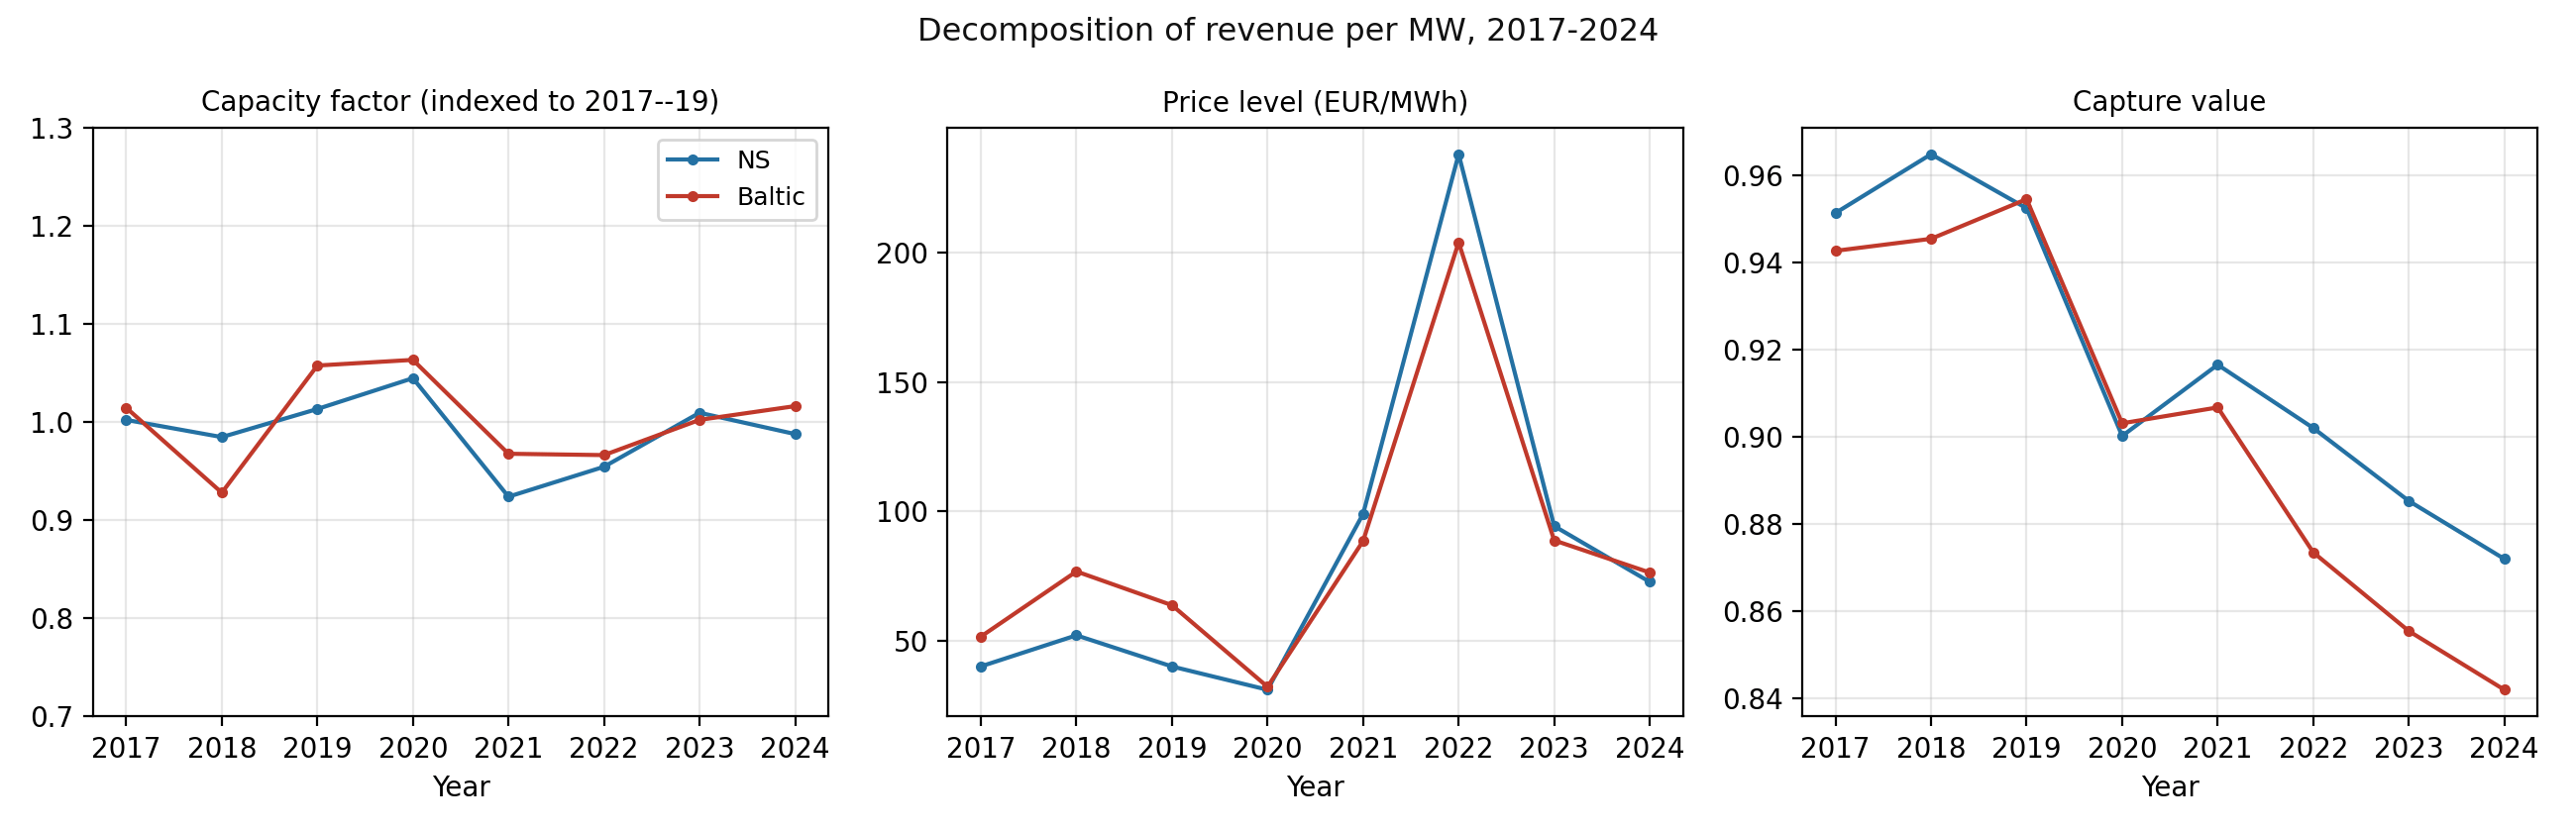
\includegraphics[width=0.98\textwidth]{fig_revenue_decomp}
    \caption{The three parts of revenue per megawatt, 2017 to 2024. Generation
    (left) is flat and the average price (centre) follows the gas crisis, while
    capture value (right) declines steadily.}
    \label{fig:revenue_decomp}
\end{figure}

Figure~\ref{fig:group_arc_observed} shows capture value for the four groups of
farms defined in Section~\ref{sec:farm_data}. Over 2023 and 2024 the Baltic
zones that have built little offshore wind capture 0.883 of the average price
and the North Sea 0.879, which puts the two level. The lower Baltic average comes from the other two
groups: DK2 and SE4, which have already built out, at 0.766, and Finland at
0.568, where nuclear generation holds prices down.

\begin{figure}[!htb]
    \centering
    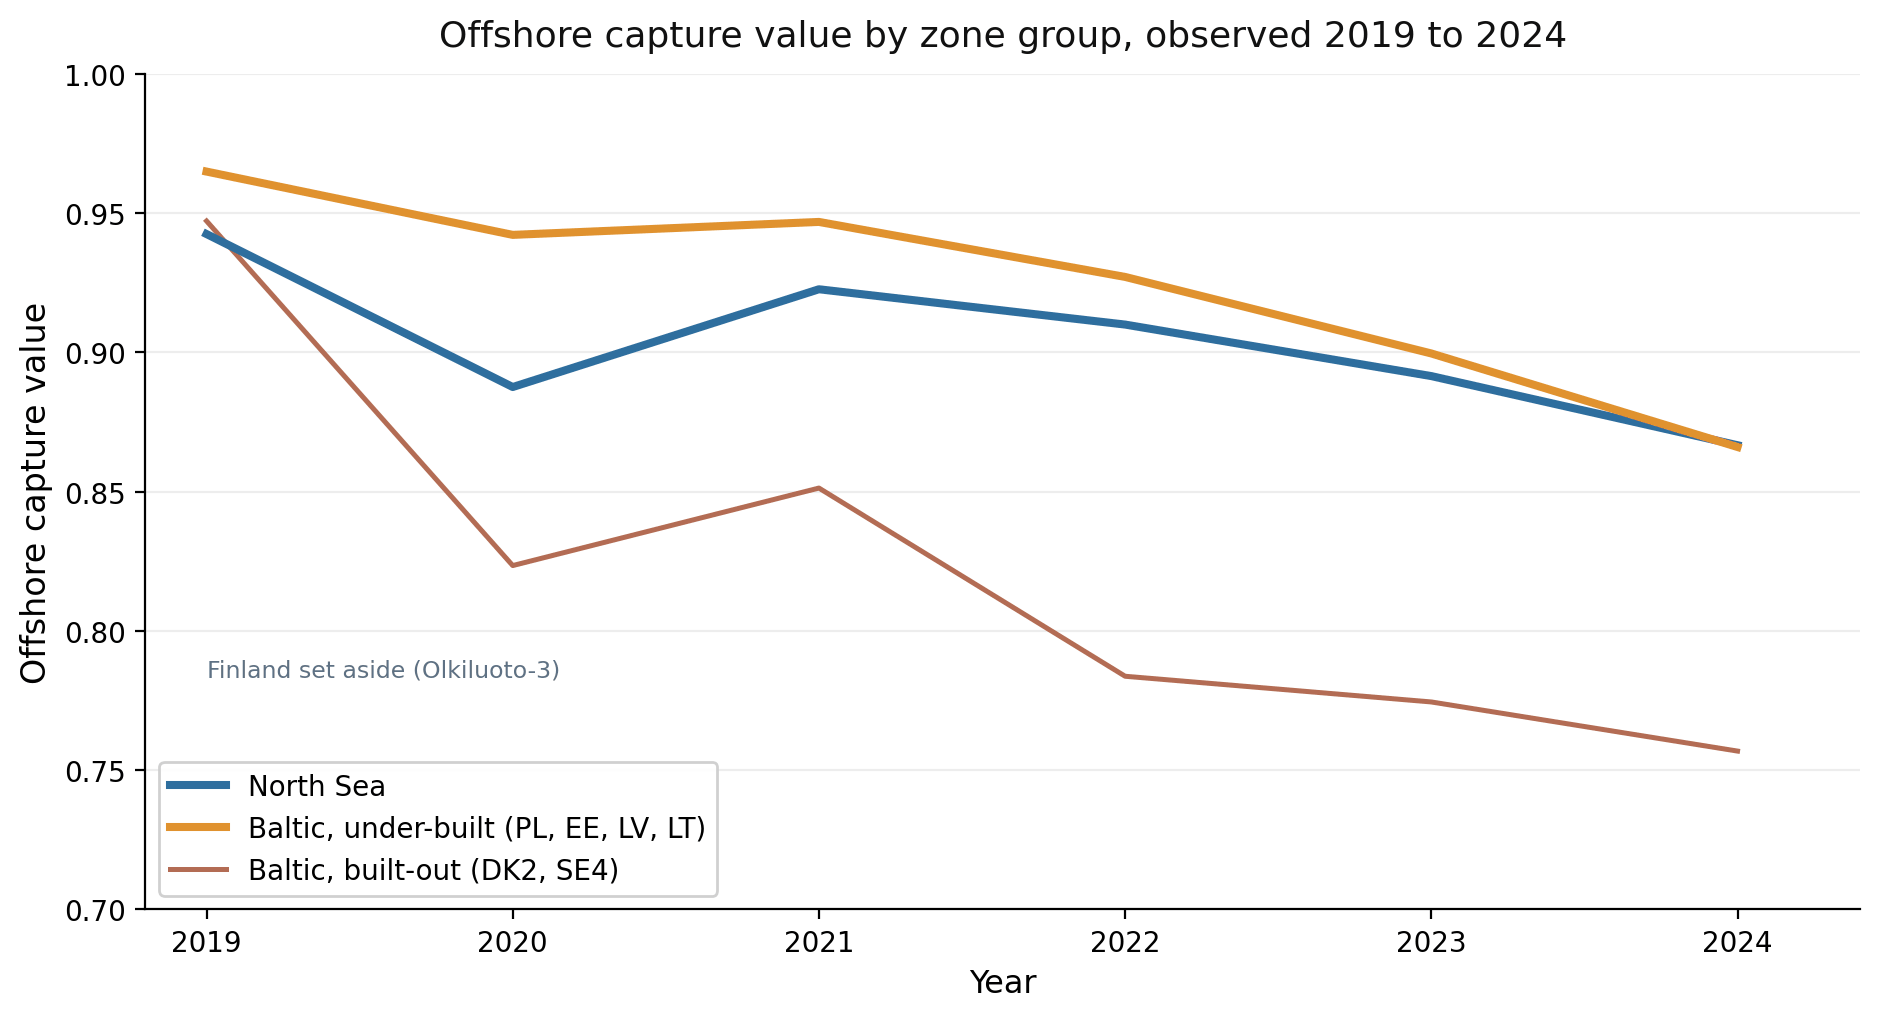
\includegraphics[width=0.9\textwidth]{fig_group_arc_observed}
    \caption{Observed capture value by group of zones, 2019 to 2024. The Baltic
    zones with little offshore wind capture the same share as the North Sea,
    while DK2 and SE4, which have built out, capture less than both.}
    \label{fig:group_arc_observed}
\end{figure}

Table~\ref{tab:archetype_measured} adds the measured values to the expectations
set out in Chapter 2, and most of those expectations are incorrect. Germany was
expected to be the most eroded market, yet its offshore farms capture 0.904. Its
offshore fleet generates at different times from its much larger onshore fleet,
and it is the onshore fleet that pulls the national figure down to 0.76
\cite{Stiewe2025}. Denmark's national 0.822 combines two very different price
zones, which are separated below.

The Baltic was expected to capture close to 1.0, above the North Sea, because
little capacity has been installed there. The measured values are level with the
North Sea. Poland captures 0.922, slightly above it. Estonia, Latvia and
Lithuania capture 0.86 to 0.88, slightly below. The group averages 0.88 against the North
Sea's 0.879, with almost none of the planned capacity built. Sweden at 0.729 and
Finland at 0.568 sit lower, but each rests on a single farm in a market
dominated by nuclear and hydro generation, where a surplus of constant output
holds prices down as much as wind does. They are read as signals about their
price zone more than about the farm, and the comparison holds without them. The
hydro premium predicted by Hirth \cite{Hirth2013} does not appear in the Baltic
after 2022.

\begin{table}[!htb]
\centering
\small
\setlength{\tabcolsep}{4pt}
\caption{Expectations from Chapter 2 compared with measurement. Measured values
are farm-level capture values for 2023 and 2024, calculated from modelled farm
output and observed zonal prices. The Swedish and Finnish rows rest on one farm
each and describe their price zone more than a typical farm, which is discussed
in Chapter 5.}
\label{tab:archetype_measured}
\begin{tabular}{l c
                >{\raggedright\arraybackslash}p{3.1cm}
                >{\centering\arraybackslash}p{1.9cm}
                >{\centering\arraybackslash}p{1.4cm}
                >{\raggedright\arraybackslash}p{3.3cm}}
\toprule
\textbf{Market} & \textbf{Basin} & \textbf{Expected in Chapter 2} &
\textbf{Measured capture value} & \textbf{Farm months} & \textbf{Outcome} \\
\midrule
Germany & NS & Eroded, declining & 0.904 & 144 & Milder than expected \\
\addlinespace
Netherlands & NS & Eroded & 0.890 & 96 & As expected \\
\addlinespace
Denmark & NS/BS & Eroded, with some buffering & 0.822 & 168 &
Averages two different zones \\
\addlinespace
Sweden & BS & Favourable (hydro) & 0.729 & 24 & Lower than expected \\
\addlinespace
Finland & BS & Favourable & 0.568 & 24 & Lower than expected, one farm \\
\addlinespace
Poland & BS & Very favourable & 0.922 & 48 & Close to expectation \\
\addlinespace
Baltic states & BS & Close to 1.0 & 0.86--0.88 & 72 &
Level with the North Sea \\
\bottomrule
\end{tabular}
\end{table}

Ordering the same zones by how much offshore wind they have built turns the
comparison into a sequence. DK2 and SE4, the most built out, capture least. The
zones with little capacity earn what the North Sea earns. The two basins are
following the same relationship between buildout and capture value,
and the Baltic entered it at the same level, with DK2 and SE4 showing the stage
it has already reached.

Two comparisons show that what sets the value is the price zone a farm sells
into. Four German farms stand in Baltic water but sell into the German market,
and they capture 0.91, the same as German farms in the North Sea. The weather is
Baltic, the market is open, and there is no discount. Denmark gives the reverse
case: DK2 captures 0.784 and DK1 0.854, in the same country and under the
same support scheme, separated only by the price zone their output must be sold
in.

That mix is what makes the Baltic average of 0.84 match no individual zone. It combines
German-priced Baltic farms at 0.91, the enclosed DK2 and SE4 at 0.78, and
Finland at 0.57. The zones with little capacity, level today, are where the
buildout starts, and the enclosed zones at 0.78 show where it leads. For those
enclosed zones, the larger part of the gap to the North Sea comes from limited
capacity to export surplus, and a smaller part from the amount of wind in the
zone itself. After the crisis the local-wind part of the gap shrank while the
interconnection and wind-pattern parts grew\label{sec:gap_opened}. These are the
same two causes measured in Section~\ref{sec:mechanism}.

% ----------------------------------------------------------------------------
\subsection{Validation of the two models}\label{sec:trust}

The supporting tables for the comparisons in this section are in
Appendices~\ref{app:reg_tables} and~\ref{app:triangle}.

\subsubsection{Performance of the regression model}\label{sec:trust_empirical}

The regression model was tested on price zones that were excluded from the
inputs used to fit it. On those zones it accounts for 69\,\% of the variation
in capture value across farms and months. Its estimates are within 0.04 of the observed value in
five of the seven enclosed Baltic zones and within 0.07 in Sweden. The one clear
miss is Finland, at 0.10, where nuclear generation holds prices down in a way
the seven market conditions used as inputs do not describe.

Measuring those conditions separately for each bidding zone, instead of once per
country, raises the score by nine points. Prices are set within zones, and
treating DK1 and DK2 as a single Danish market would hide the difference between
them, which is central to this thesis.

The model's limit emerges once it is fitted on data up to 2022 and asked to
estimate 2023 and 2024, where it performs worse than simply assuming that every farm
has the average capture value. The energy crisis pushed gas and carbon prices
beyond anything in its training data. Leaving out one year at a time confirms
this: the model works well inside the range of conditions covered by its
training inputs, and fails across the break between 2021 and 2022.

\subsubsection{Performance of the system model}\label{sec:trust_system}

The system model is solved with the transmission grid held at its present
capacity, so congestion is priced as it exists today. This makes the absolute
price level less accurate, which matters little in this case. Capture value is a ratio
between the price a farm earns and the average price in its market, so an error
shared by both largely cancels.

Where the grid is strong the ratio matches observation closely. In Germany the
model gives 0.908 against an observed 0.909, and the Netherlands is similar.
Where the grid is congested the model reads too high, and the gap widens as
congestion increases: 0.03 too high in Belgium and 0.06 in DK1. These are
differences in capture value itself, so 0.06 means the model credits Danish
offshore farms with six per cent more of the average price than they earned.
Great Britain and Norway do not pass this check at the resolution used and
are excluded from every aggregate.

Because the model's error runs in one direction only, always crediting farms
with more of the average price than they received, it is a bias in the
statistical sense, and a bias can be traced to its source. The model produces
two outputs that could carry it, the generation of each farm and the price in
each hour, and the two are separated by valuing the model's own generation at
the prices that were actually observed. Most of the error disappears under
that substitution, which shows that the modelled generation is close to
correct and that the bias sits in the modelled prices. The same bias appears
again in 2019 and in 2024, so it is stable from year to year, and an error
that is stable and always in one direction can be measured and subtracted,
which is what the correction of Section~\ref{sec:bias_method} does.

The one zone that cannot be corrected is DK2, where the model reads 0.14 too
high. That zone
had 264 hours of negative prices in 2023, which occur because some plants keep
running even when prices are below zero: combined heat and power stations that
must supply heat, and generators whose subsidy makes it worth paying to stay
online. The system model is a linear optimisation and does not represent
decisions of that kind, so it produces no negative prices at all. This
limitation belongs to the class of model, so DK2 is set aside
(Appendix~\ref{app:robustness}).

\subsubsection{Allocation of models to analytical tasks}\label{sec:division}

When the two models are compared with the same observed record, the regression
model proves the more accurate of the two: across fifteen combinations of
price zone and year, its estimates deviate from the observed capture value by
0.011 on average, against 0.054 for the system model. A difference in this
direction is expected from the way each model is estimated. The regression
model is fitted to the observed prices themselves, so it reproduces market
behaviour that a cost-based simulation cannot, including the hours in which
the price falls below zero. The system model instead derives its prices from
generation costs, and observed prices depart from cost-based prices whenever
something the model does not represent intervenes, such as a plant that must
keep running or a sudden movement in fuel prices. For measuring the present
and the recent past, the regression model is therefore the more reliable
instrument, and the question that remains is whether the same holds beyond the
observed record.

Each model
is used where the evidence supports it. The regression model measures
the present, explains why one farm earns less than another, and supports
short-term projection. The system model carries the projection to 2030 and 2040,
because it derives its prices from costs, and because it
alone can be solved again under a different grid, gas price or level of
flexibility (Table~\ref{tab:model_verdict}).

\begin{table}[!htb]
\centering\small
\setlength{\tabcolsep}{4pt}
\caption{Comparison of the two models across the six tasks the thesis requires
of them. Errors are average deviations from observed capture value over the
fifteen zone-year validation points of Appendix~\ref{app:triangle}; scenario
ranges are measured across the four Baltic 2040 scenarios.}
\label{tab:model_verdict}
\begin{tabular}{>{\raggedright\arraybackslash}p{2.2cm}
                >{\raggedright\arraybackslash}p{3.2cm}
                >{\raggedright\arraybackslash}p{6.9cm}
                >{\raggedright\arraybackslash}p{1.9cm}}
\toprule
\textbf{Question} & \textbf{Task} & \textbf{Result} & \textbf{Conclusion} \\
\midrule
Accuracy on the observed record &
Reproduce the capture value observed between 2017 and 2024 &
The regression model deviates from observation by 0.011 on average and the
system model by 0.054, with the system model's error growing with congestion &
Regression model \\
\addlinespace
The most cannibalised zone &
Reproduce DK2 in 2023, where 0.784 was observed &
The regression model gives 0.798, an error of 0.014, while the system model
gives 0.932, an error of 0.148 &
Regression model \\
\addlinespace
Negative prices &
Reproduce hours in which the price falls below zero &
The regression model learned these hours from observed prices, while the
system model builds prices from generation costs, which cannot fall below
zero &
Regression model \\
\addlinespace
Congestion &
Represent congestion and flows between countries &
The regression model carries them only as input variables, while the system
model computes a price at every grid node, so congestion appears directly &
System model \\
\addlinespace
Conditions beyond the record &
Estimate capture value at renewable shares beyond the historical record &
Across the four 2040 scenarios the regression model's answers span only 0.008,
while the system model's span 0.428 and respond to the buildout &
System model \\
\addlinespace
Changed assumptions &
Estimate the effect of a different grid, gas price or level of flexibility &
The regression model contains no representation of the power system to change,
while the system model is solved again with the assumption changed &
System model \\
\bottomrule
\end{tabular}
\end{table}
\FloatBarrier
\subsection{Sources of divergence between the models}\label{sec:why_differ}

Section~\ref{sec:trust} establishes where each model can be trusted. This
section explains why they differ, since passing the projection from one model to
the other is only defensible if the difference is understood. The full
arithmetic is in Appendices~\ref{app:triangle} and~\ref{app:forecast_checks}.

\subsubsection{Agreement within the observed record}\label{sec:gap_decomposition}

Over the four zones the 2023 record can check, the two models give almost the
same answer: 0.890 against 0.885 in capture value, a difference of 0.005. Two
models that share no code, one learning from eight years of observed prices and
one rebuilding prices from generation costs, land within half a point of each
other. Zone by zone the agreement is looser, with differences running from 0.001
at Belgium to 0.056 at DK1.

The two models differ in only two inputs, the generation series each uses and
the prices each applies to it, so the difference between their answers can be
split between those two causes. Both parts are small, and one adds while the
other subtracts. The generation part adds 0.004, because the system model's
output is smoother than a farm-specific weather series, and a smoother profile
earns slightly more of the average price. The price part subtracts 0.014,
because the system model's prices stay flatter across windy hours and so
understate how far prices fall when wind blows. The way the network is
represented adds 0.004 on average, and 0.050 at DK1 alone. Forbidding negative
prices is the largest structural difference between the two models, and it
changes the answer least, at 0.003, because the 221 to 315 negative hours
observed are too few to move a yearly average.

\subsubsection{Out-of-sample skill and the choice of model}\label{sec:skill}

Both models were applied to the same Baltic zones with only the projection
year changed, and their estimates differ by 0.035 in 2030 and by 0.348 in
2040, ten times as much. The widening has an identifiable source in the scope
of the regression model's training inputs. In 2030 the assumed market
conditions still lie within the range covered by those inputs, so the 0.035 is
a genuine disagreement between the models about how prices form, whereas by
2040 the conditions have moved outside that range and the regression model
returns almost the same estimate regardless of the scenario assumptions. This
loss of response accounts for 0.313 of the 0.348, so ninety per cent of the
2040 difference arises because one model has stopped responding to its inputs.

Which assumption pushes the regression model outside its range can be
identified, because the scenarios vary four inputs. Of the four, only the
share of electricity generated by renewables moves far beyond the training
data, rising to roughly fifteen times today's level in the Baltic, and on this
input alone fourteen of the thirty-six projected cases fall outside the range
the model was fitted on, while a check across all seven market conditions
together places all thirty-six outside it. Repeating the projection with the
carbon price held at its highest observed value leaves the estimates
unchanged, which rules carbon out and identifies renewable share as the
binding assumption\label{sec:two_estimators}.

Judged month by month over the years already observed, the two models are
equally accurate. Both were scored on 144 combinations of price zone and month
that neither had been built from. The regression model is out by 0.041 in
capture value on average and the system model by 0.046, a gap too small to be
meaningful given how few independent price zones there are. This sits
oddly beside the annual comparison of Section~\ref{sec:division}, where the
regression model was five times closer, and the reason is the averaging. The
regression model's error is in which months are high and which are low, and
those errors cancel once a year is averaged.

What separates them is the kind of mistake each model makes
(Table~\ref{tab:skill}). The system model reads too high almost every time, by
0.041 on average, and an error that always points the same way can be measured
and subtracted, which is what the correction in Section~\ref{sec:bias_method}
does. The regression model reads slightly low, and its error is the mistiming
described above, for which there is no single number to subtract.

Fitted on nothing after 2021 and asked for 2023 and 2024, the two models are
again equally accurate, at 0.049 each, because those two years still lay largely
within the conditions the regression model had learned from
(Appendix~\ref{app:forecast_checks})\label{sec:backtest}.

\begin{table}[!htb]
\centering\small
\caption{Error composition of the two models on 144 zone-months withheld from
both, in units of capture value; a positive bias means the model reads high.
The full decomposition is in Appendix~\ref{app:forecast_checks}.}
\label{tab:skill}
\begin{tabular}{l c c l}
\toprule
\textbf{Model} & \textbf{Average error} & \textbf{Bias} &
\textbf{Where the error comes from} \\
\midrule
Regression model, tested on zones it never saw & 0.041 & $-0.026$ &
Which months are high and which are low \\
Regression model, tested on years it never saw & 0.046 & $-0.018$ &
Which months are high and which are low \\
System model & 0.046 & $+0.041$ & Reading too high in almost every case \\
\bottomrule
\end{tabular}
\end{table}
\FloatBarrier

The projection of Section~\ref{sec:projection_results} therefore uses the system
model, with the correction applied to it as a
refinement\label{sec:external}.

\subsection{Projected capture value under the committed buildout, using the system model}
\label{sec:projection_results}

Sections~\ref{sec:trust} and~\ref{sec:why_differ} established that the system
model is the one that can be used beyond the observed record. This section uses
it to project capture value forward, as the offshore wind already planned around
the two seas is built. The capacities are those of the 2024 Ten-Year Network
Development Plan, so this is the buildout that governments and system operators
have already committed to, and the projection runs to 2030 and 2040. The values
reported are those the system model produces directly. The correction of
Section~\ref{sec:bias_method} is applied afterwards as a refinement.

The projected values depend on the whole power system around each farm, so
Figure~\ref{fig:energy_mix} shows the installed capacity assumed at each year.

\begin{figure}[!htb]
    \centering
    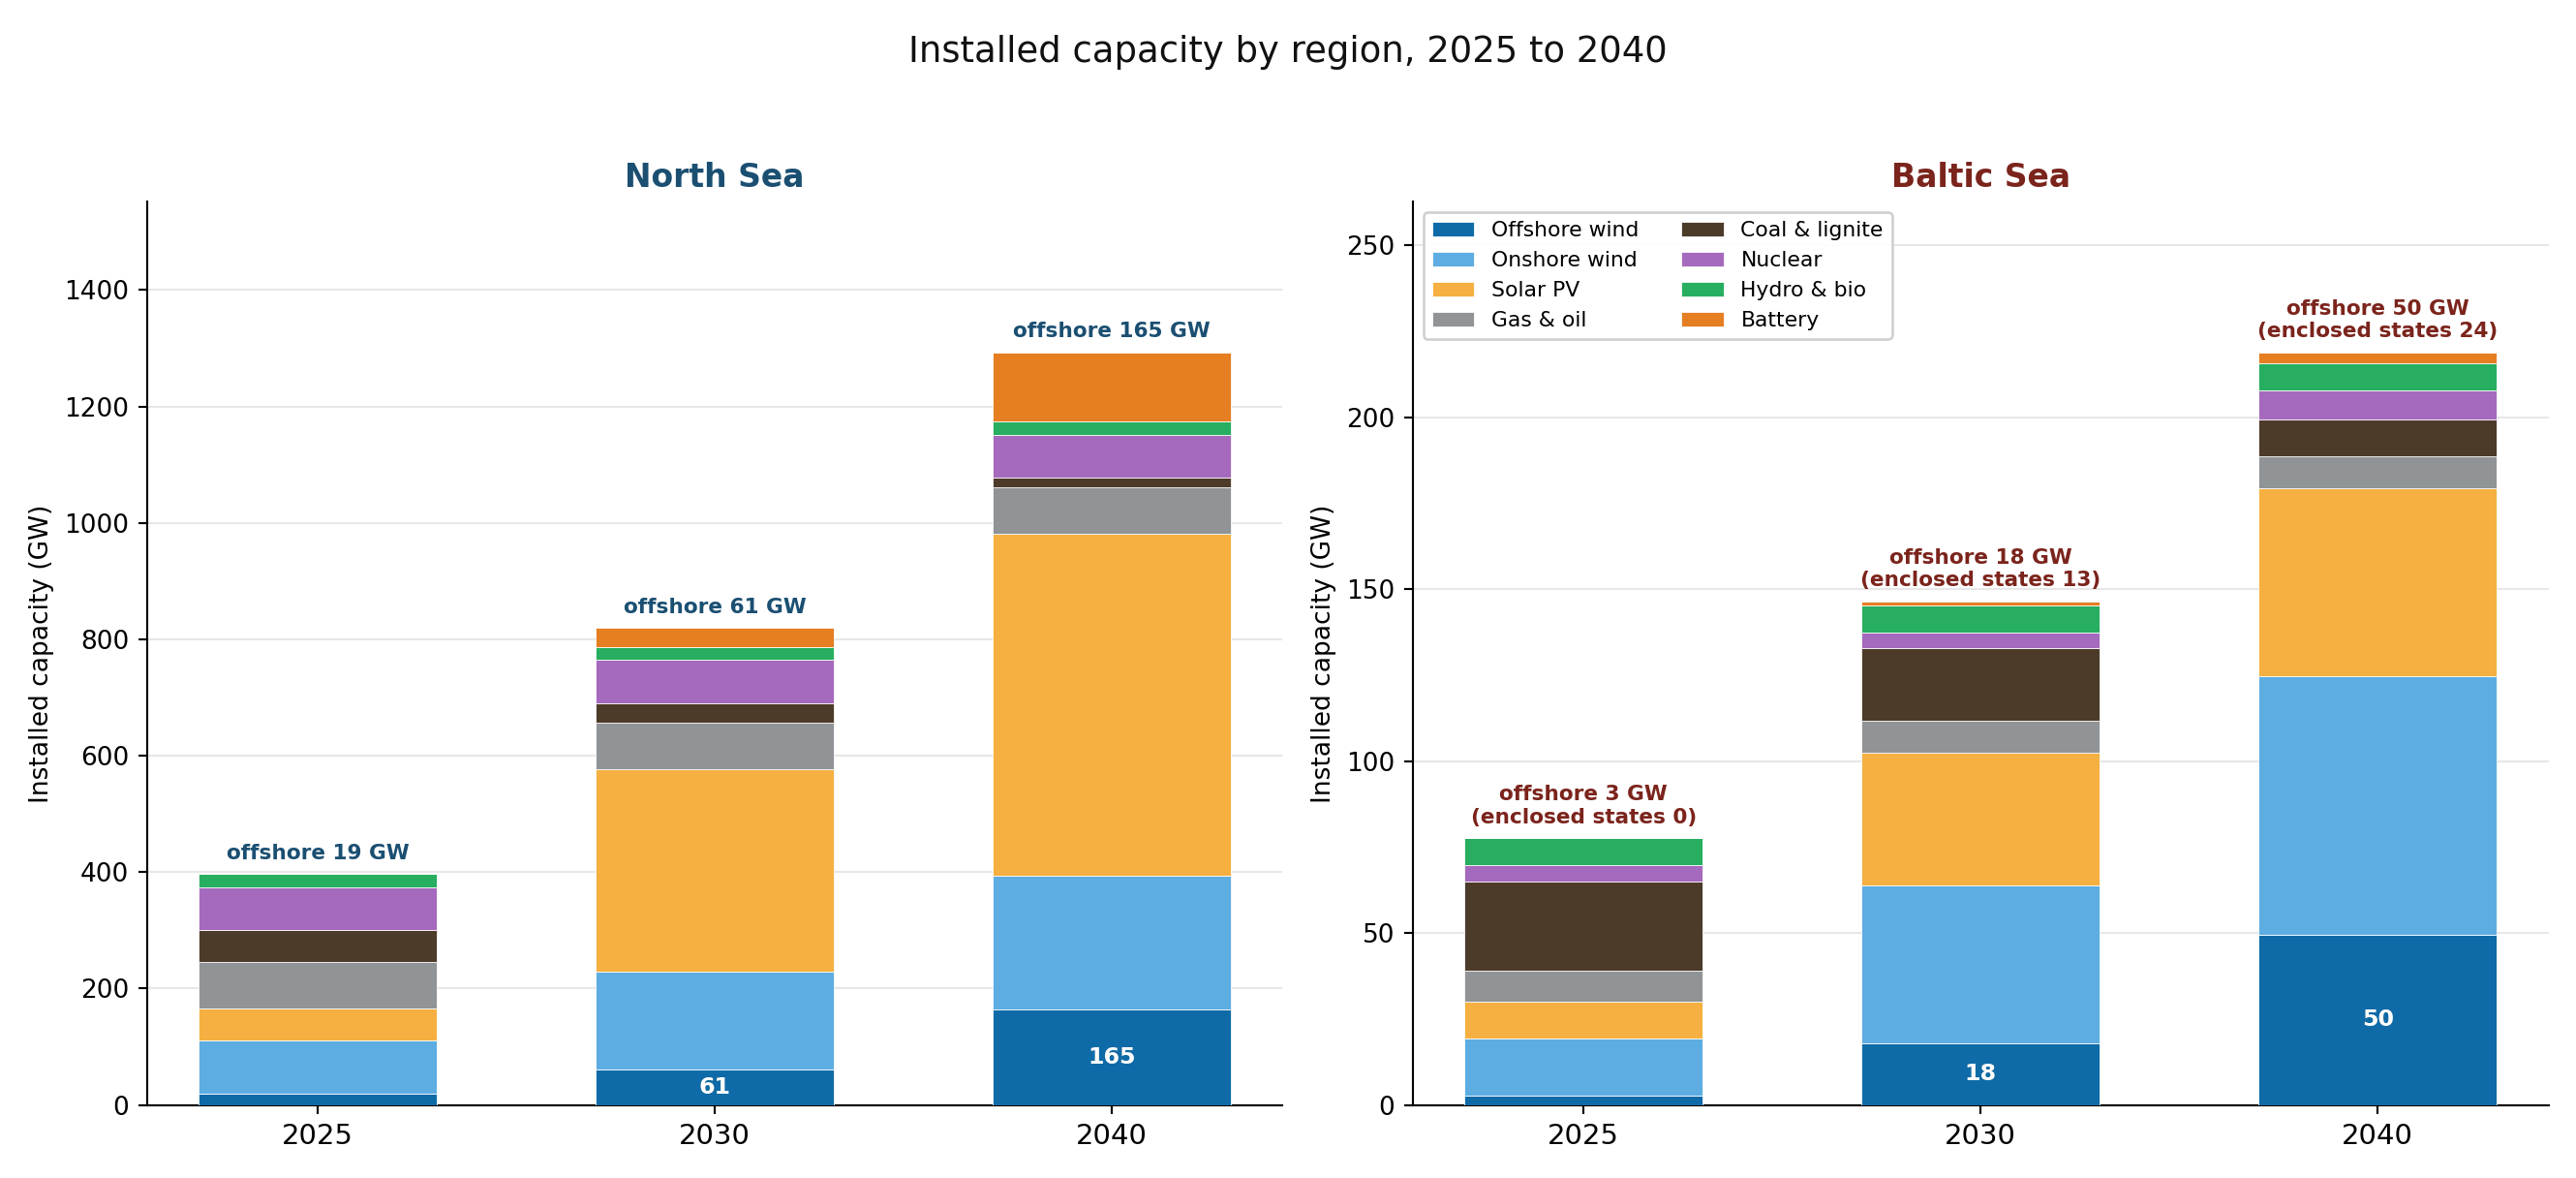
\includegraphics[width=0.95\textwidth]{fig_energy_mix}
    \caption{Installed capacity to 2040 under the TYNDP trajectories. Offshore
    wind is assigned to the sea each farm stands in, and all other capacity to
    the fleet of the bordering region.}
    \label{fig:energy_mix}
\end{figure}

Around the North Sea, offshore wind grows from 18.5 to 164.8~GW, nine times its
present size. Around the Baltic it grows from 2.6 to 49.5~GW, nineteen times its
present size. The Baltic starts much smaller and grows twice as fast, and that
difference drives the results below.

What stays in the system matters as much as what is added. Gas, nuclear and
hydro capacity remain at similar levels in all three years, and only coal
declines. Wind costs almost nothing to run once it is built, so in windy hours
it pushes the wholesale price down. In hours with little wind, gas and other
conventional plants are still needed and still set the price. Capture value
falls because more and more wind output arrives in the hours when wind has
already pushed the price down.
\subsubsection{Projected capture value to 2030 and 2040}\label{sec:corrected_projection}

The system model was solved for six scenarios from the 2024 Ten-Year Network
Development Plan, listed in Table~\ref{tab:projection}. They cover 2030 and
2040, a scheduled and an accelerated pace of Baltic buildout, and the plan's
three demand pathways. National Trends, the pathway that tracks existing
national policies, is the one quoted in the text, and the table gives the
rest. Finland is set aside, as in the measured record.

Baltic capture value falls steeply under National Trends, from 0.88 today to
0.47 by 2040, while the North Sea holds 0.57, and most of the fall arrives
after 2030. The faster the Baltic builds, the further it
falls: in the accelerated case it reaches 0.36. These values come from the
model directly, with no correction applied, and in every 2040 scenario the
Baltic ends below the North Sea.

Applying the correction for the overstatement measured in
Section~\ref{sec:trust_system} (the model reads too high in congested zones)
deepens each 2040 value by roughly a further 0.1. The correction is a
refinement, and the conclusion does not depend on it, since its size rests
almost entirely on DK2, and removing that zone leaves a nearly constant
adjustment (Appendix~\ref{app:robustness}). Where a single number is needed,
this thesis uses 0.47, the uncorrected National Trends case on today's grid,
at which the Baltic has lost close to half of its present value.

Two further checks leave this conclusion unchanged, as expanding the
transmission grid softens the fall without undoing it
(Section~\ref{sec:grid_results}) and the assumed level of hydrogen demand
barely moves it. The basin average also
conceals differences between zones, with Estonia falling furthest and Poland
least (Appendix~\ref{app:tables}), but every zone that builds out loses value.

\begin{table}[!htb]
\centering\small
\caption{Projected capture value by scenario, averaged across each basin and
weighted by generation, from the system model with the transmission grid held
at today's capacity and no correction applied. The corrected Baltic values are
in Appendix~\ref{app:robustness}; Finland is set aside throughout.}
\label{tab:projection}
\begin{tabular}{c l l c c c}
\toprule
\textbf{Year} & \textbf{Demand pathway} & \textbf{Baltic buildout} &
\textbf{Baltic offshore} & \textbf{North Sea} & \textbf{Baltic} \\
 & & & \textbf{share of consumption} & \textbf{capture value} &
\textbf{capture value} \\
\midrule
2030 & National Trends & scheduled & 0.24 & 0.84 & 0.79 \\
2030 & National Trends & accelerated & 0.29 & 0.84 & 0.75 \\
\addlinespace
2040 & National Trends & scheduled & 0.33 & 0.57 & 0.47 \\
2040 & National Trends & accelerated & 0.51 & 0.57 & 0.36 \\
2040 & Distributed Energy & accelerated & 0.38 & 0.63 & 0.60 \\
2040 & Global Ambition & accelerated & 0.40 & 0.70 & 0.57 \\
\bottomrule
\end{tabular}
\end{table}
\subsubsection{Spatial distribution of projected capture value}\label{sec:maps}

Figure~\ref{fig:heatmap_2040} shows the capture value a farm would earn at each
buildable location in 2040. The 2025 and 2030 maps are in
Appendix~\ref{app:reg_tables}.

\begin{figure}[!htb]
    \centering
    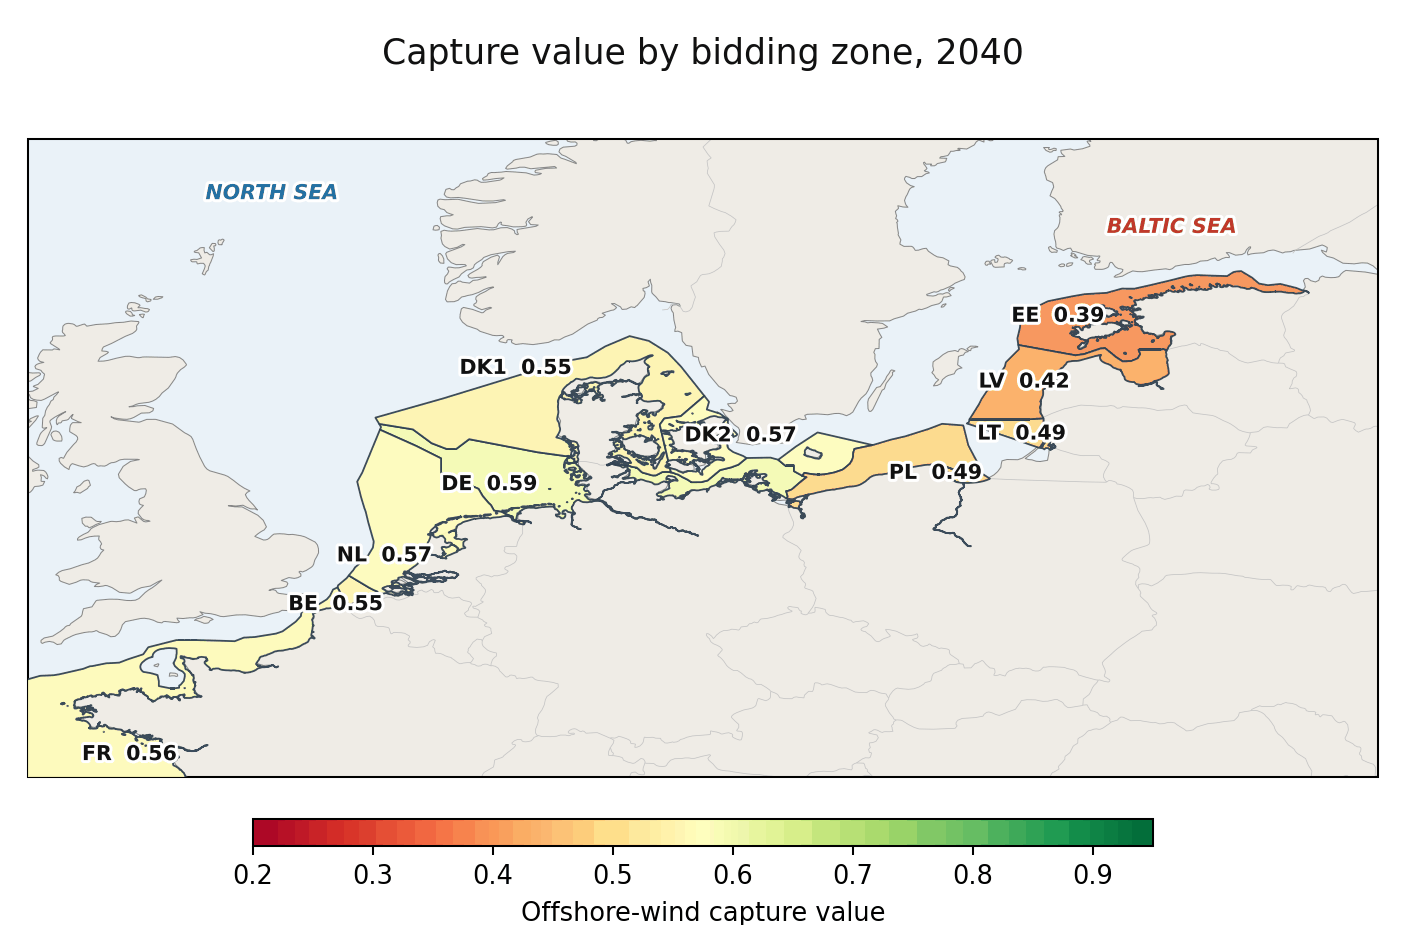
\includegraphics[width=0.80\textwidth]{fig_heatmap_2040}
    \caption{Capture value at each buildable location in 2040, with the
    transmission grid held at today's capacity. The North Sea holds close to its
    present level, while the enclosed eastern Baltic falls furthest.}
    \label{fig:heatmap_2040}
\end{figure}

In 2025 capture value is high and much the same across the whole shelf. By 2030
it has fallen everywhere, with no clear difference between the two seas. By 2040
the two have separated: the eastern Baltic is lowest, while the North Sea holds
its level despite taking far more new capacity. What decides the fall is how
easily a basin can move its surplus away.

Appendix~\ref{app:atlas} repeats these maps under cost-optimal transmission,
alongside levelised cost, value-adjusted cost, net value and revenue density at
all three years. Comparing the frozen and expanded versions shows the split of
Section~\ref{sec:decomposition} geographically.
\FloatBarrier


% ----------------------------------------------------------------------------
\FloatBarrier
\subsection{Drivers of value erosion and its recoverable component}\label{sec:mechanism}

This section examines what drives the fall in capture value and how much of it
depends on the configuration of the surrounding system. The first part
identifies what sets the severity of the fall: the differences between
individual farms, the shape of the relationship between buildout and value,
and the season in which the loss concentrates. The second part quantifies that
dependence, by re-solving the scenarios with transmission free to expand and
by decomposing the fall into a congestion component and a structural
component.

Three further checks are reported in Appendix~\ref{app:robustness}. The same
geography appears from hourly generation alone, with no prices used at all.
Removing the hours priced by scarcity leaves the fall largely intact. And
allowing demand to shift in time recovers as much capture value as expanding the
grid does.

\subsubsection{Farm-level drivers}\label{sec:shap_results}

This part asks why one farm earns less than another in the same month. Carbon
and gas prices cannot explain it: they are Europe-wide monthly prices, identical
in every zone, so they move all farms together. They still appear important in
the fitted model, because the 2021 to 2022 fuel crisis moved fuel prices and
capture value at the same time.

Comparing each farm with the average of all farms in the same month removes that
common movement (Figure~\ref{fig:shap}). Carbon's share then falls from 29 to
4\,\% and gas from 14 to 3\,\%. Crowding takes their place: how closely a farm's
output follows the wind of the system around it explains 32\,\% on its own, and
the zone's existing wind capacity a further 13\,\%. A farm generating when
everything else is generating sells into a market already full of wind, and that
is the largest single cause of a low capture value.

The rest is the system's ability to absorb that surplus. How well demand matches
generation, how much flexibility exists, and how much can be exported together
explain about 48\,\%, each by moving surplus out of the windiest hours, either
across a border or into storage. The Baltic, with less export
capacity, is the more exposed basin. Fuel prices still set the overall price
level, but the differences between farms come from crowding and from how much
surplus the system can absorb.

\begin{figure}[!htb]
    \centering
    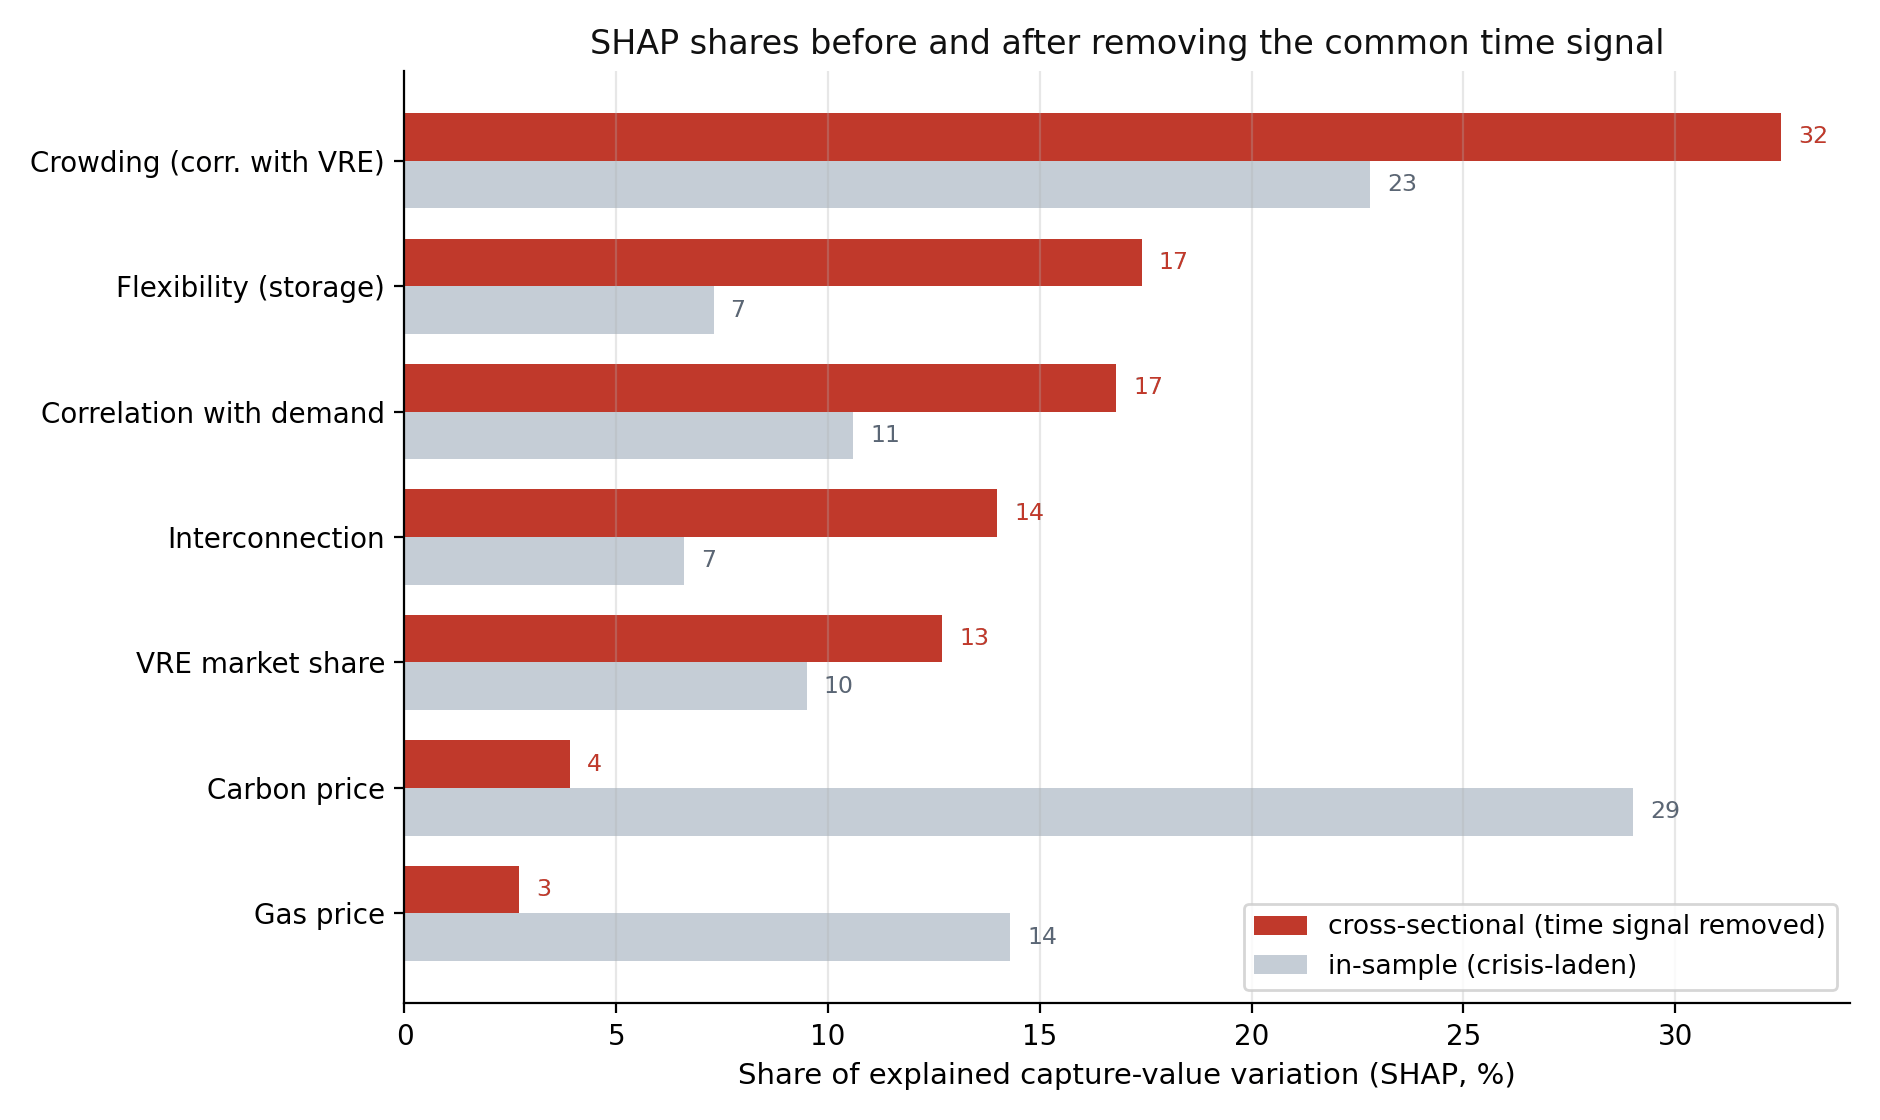
\includegraphics[width=0.95\textwidth]{fig_shap_demeaned}
    \caption{Importance of each driver of capture value, measured by SHAP.
    Grey shows the values as fitted; red shows them after each farm is
    compared with the average of all farms in the same month, which removes
    movements common to every zone.}
    \label{fig:shap}
\end{figure}

A much simpler equation, fitted separately to each basin, checks this result
(Equation~\ref{eq:analytical}). One term in it measures how heavily a farm is
penalised for generating at the same time as everything else. That penalty is
0.74 in the Baltic against 0.37 in the North Sea, and the Baltic is the steeper
of the two in 99 of 100 resamplings of the farms. Capture value falls
about 1.6 times as fast per unit of buildout in the Baltic as in the North Sea
today, and about 1.9 times as fast once wind dominates the system. Fifteen farms
is a small basis, so this is indicative, but it agrees with the system model,
which shows a moderate fall by 2030 and a severe one by 2040. The fit is in
Appendix~\ref{app:analytical}\label{sec:one_equation}.
\subsubsection{Seasonality of the erosion}\label{sec:seasonality}

Wind in the two basins peaks together in winter and separate in summer
(Figure~\ref{fig:crossbasin_sync}). Their output moves together at a correlation
near 0.4 in winter, falling to 0.13 in July. The Baltic can therefore export its
surplus in summer, but not in winter, when the same Atlantic weather reaches
both seas. Export capacity is least useful in the season when output is highest.

\begin{figure}[!htb]
    \centering
    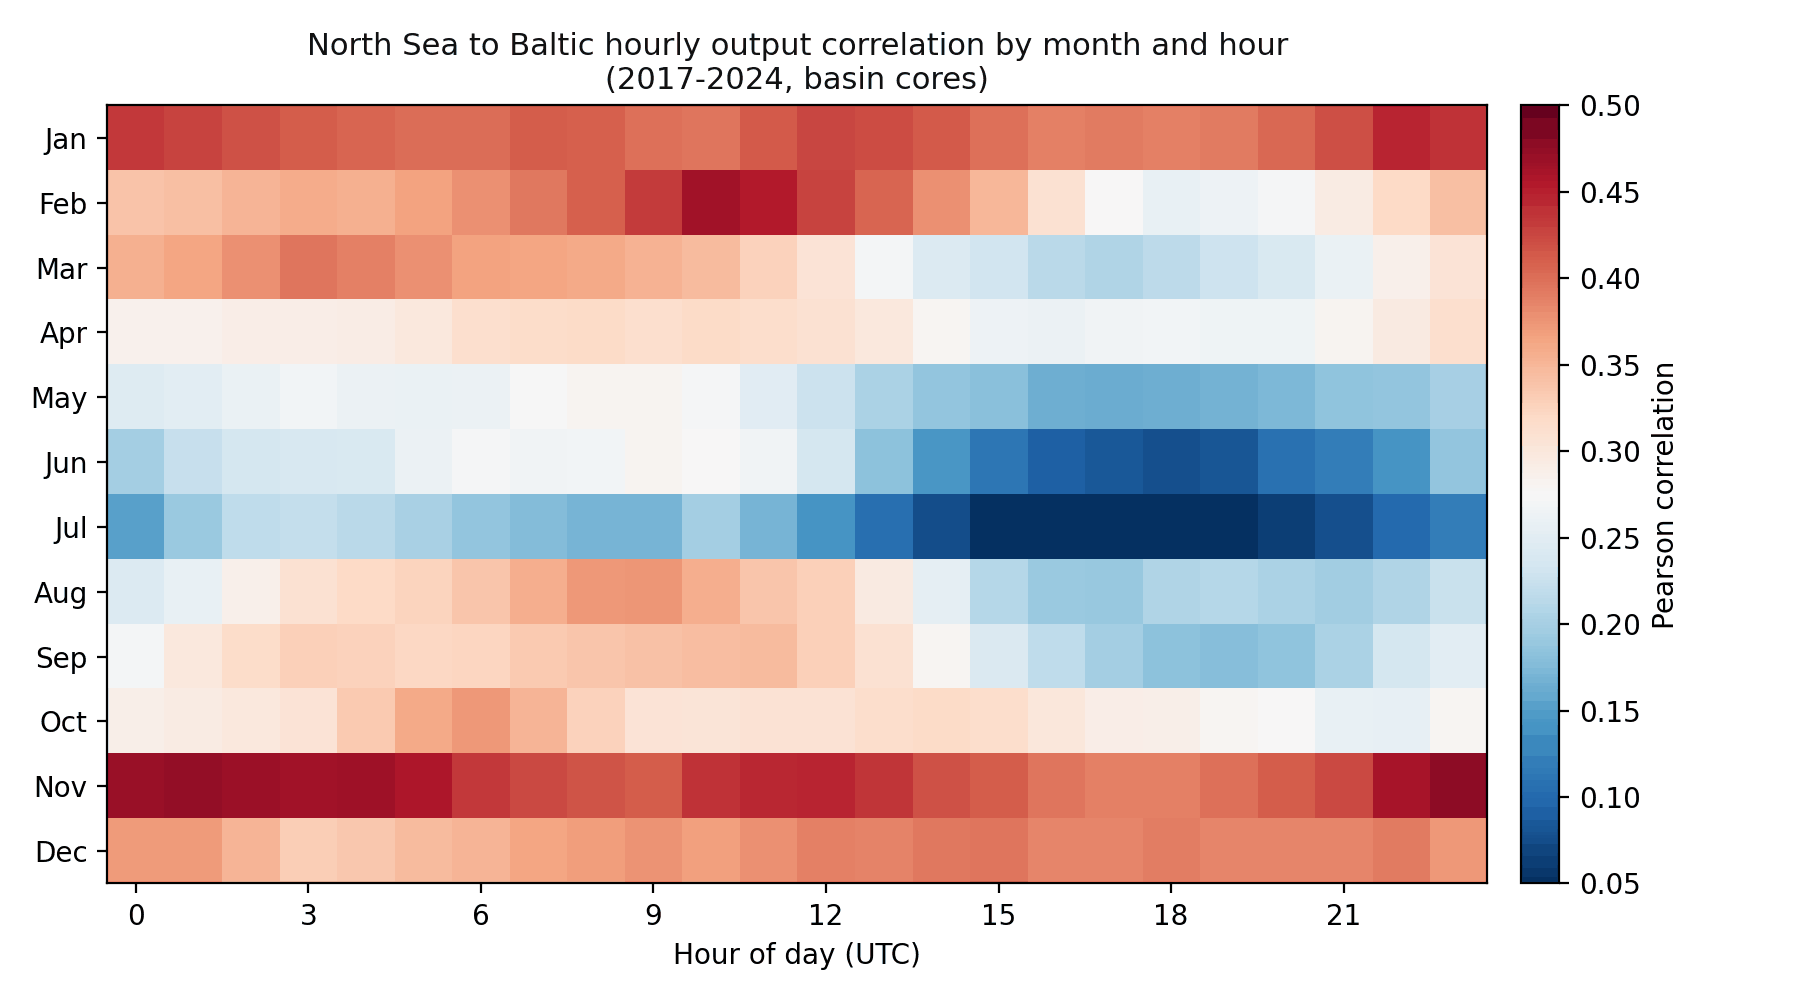
\includegraphics[width=0.95\textwidth]{fig_crossbasin_sync}
    \caption{How closely wind output in the two basins moves together, by month
    and hour, 2017 to 2024. The correlation averages 0.38 in winter and 0.20 in
    summer, and is lowest on summer afternoons.}
    \label{fig:crossbasin_sync}
\end{figure}

That matters because winter is when the farms generate, at about 70\,\% of
capacity against 40\,\% in summer, yet today they record the same capture value
in both seasons. By 2040 the loss falls almost entirely in winter, to 0.56 in the
North Sea and 0.50 in the Baltic, while summer stays at 0.91 and 0.83
(Figure~\ref{fig:seasonal_generation}, Appendix~\ref{app:supplementary}). Most
of the year's output arrives in winter, so the winter fall is what produces the
annual one, and any remedy must work in that season: interconnection, seasonal
storage, or demand that can shift into windy winter hours.

\subsubsection{The effect of transmission expansion}
\label{sec:grid_results}

The projection so far holds the grid at today's capacity, which is a
pessimistic assumption, since transmission will be built over the fifteen
years to 2040. To find the opposite bound, all six scenarios were solved again
with transmission free to expand wherever doing so lowers total system cost
(Figure~\ref{fig:grid_bracket}).

Expansion changes nothing at 2030, because the congestion it would relieve has
not yet appeared. By 2040 it matters a great deal. Under National Trends the
Baltic recovers from 0.47 to 0.66 while the North Sea moves from 0.57 to 0.64,
so the basin that trails on today's grid ends slightly ahead once the grid is
expanded. Every Baltic zone shares in the gain, Poland most of all. 

Two conclusions follow from this comparison: the Baltic's disadvantage
relative to the North Sea is largely attributable to congestion and disappears
once transmission is expanded, whereas its loss relative to its own present
value persists under either grid assumption, since the fall from 0.88 today is
severe in both.

\begin{figure}[H]
    \centering
    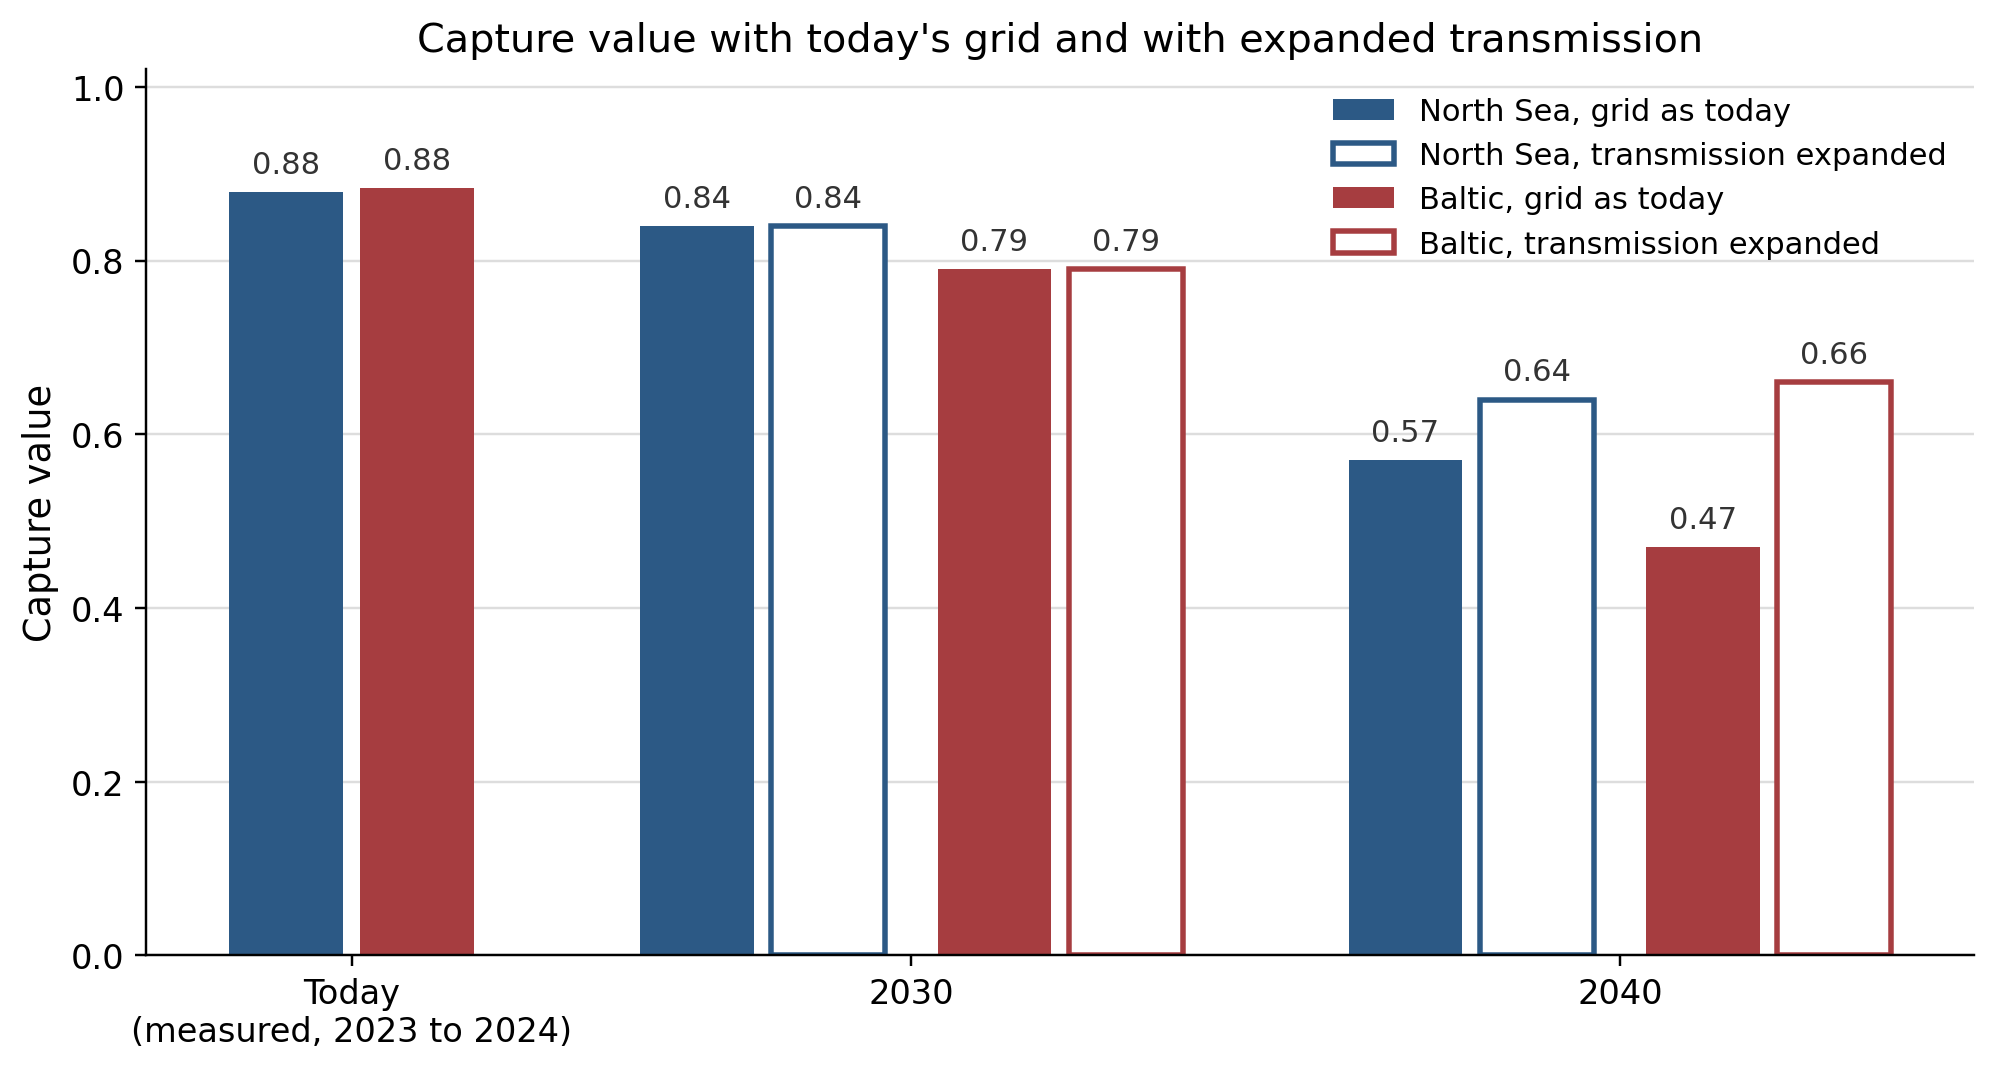
\includegraphics[width=0.9\textwidth]{figures/image-1787752046559.png}
    \caption{Capture value in both basins with the grid held at today's
    capacity and with transmission free to expand, under National Trends with
    the scheduled buildout. The bars for today are the measured 2023 to 2024
    values, where only one grid exists. Expansion makes no difference in 2030,
    and by 2040 it lifts both basins, the Baltic by more, because its loss is
    mostly congestion. Values are from the model before the bias correction,
    which is applied in the text.}
    \label{fig:grid_bracket}
\end{figure}

\subsubsection{Decomposition into congestion and structural components}\label{sec:decomposition}

The previous section establishes that transmission expansion matters, but it
does not establish how much of the total fall congestion accounts for. That
share is the number the policy conclusion rests on, because the congestion
part of the fall can be removed by building lines, while the part caused by
the buildout itself remains whatever is built.

The two model runs already provide this separation, since today's observed
capture value is the starting point, the run with transmission free to expand
gives the value a basin would hold if the grid were never a constraint, and
the run with the grid frozen gives the value it holds now. The fall between today and 2040 therefore divides
in two:
%
\begin{equation}
    \underbrace{\mathrm{CV}_{\text{today}} - \mathrm{CV}_{\text{frozen}}}_{\text{total fall}}
    = \underbrace{\bigl(\mathrm{CV}_{\text{today}} - \mathrm{CV}_{\text{optimal}}\bigr)}_{\text{structural, which no grid removes}}
    + \underbrace{\bigl(\mathrm{CV}_{\text{optimal}} - \mathrm{CV}_{\text{frozen}}\bigr)}_{\text{congestion, which an expanded grid removes}}
    \label{eq:cv_decomposition}
\end{equation}

Both basins start level, at 0.887 in the North Sea and 0.889 in the Baltic,
within half a point of the measured 0.879 and 0.883. By 2040 on the frozen grid
the North Sea has fallen by 0.314 and the Baltic by 0.418. Of the North Sea's
fall, 0.250 is structural and 0.064 is congestion, a split of 80 to 20. Of the
Baltic's, 0.225 is structural and 0.193 is congestion, a split of 54 to 46
(Figure~\ref{fig:cv_decomposition}).

\begin{figure}[!htb]
    \centering
    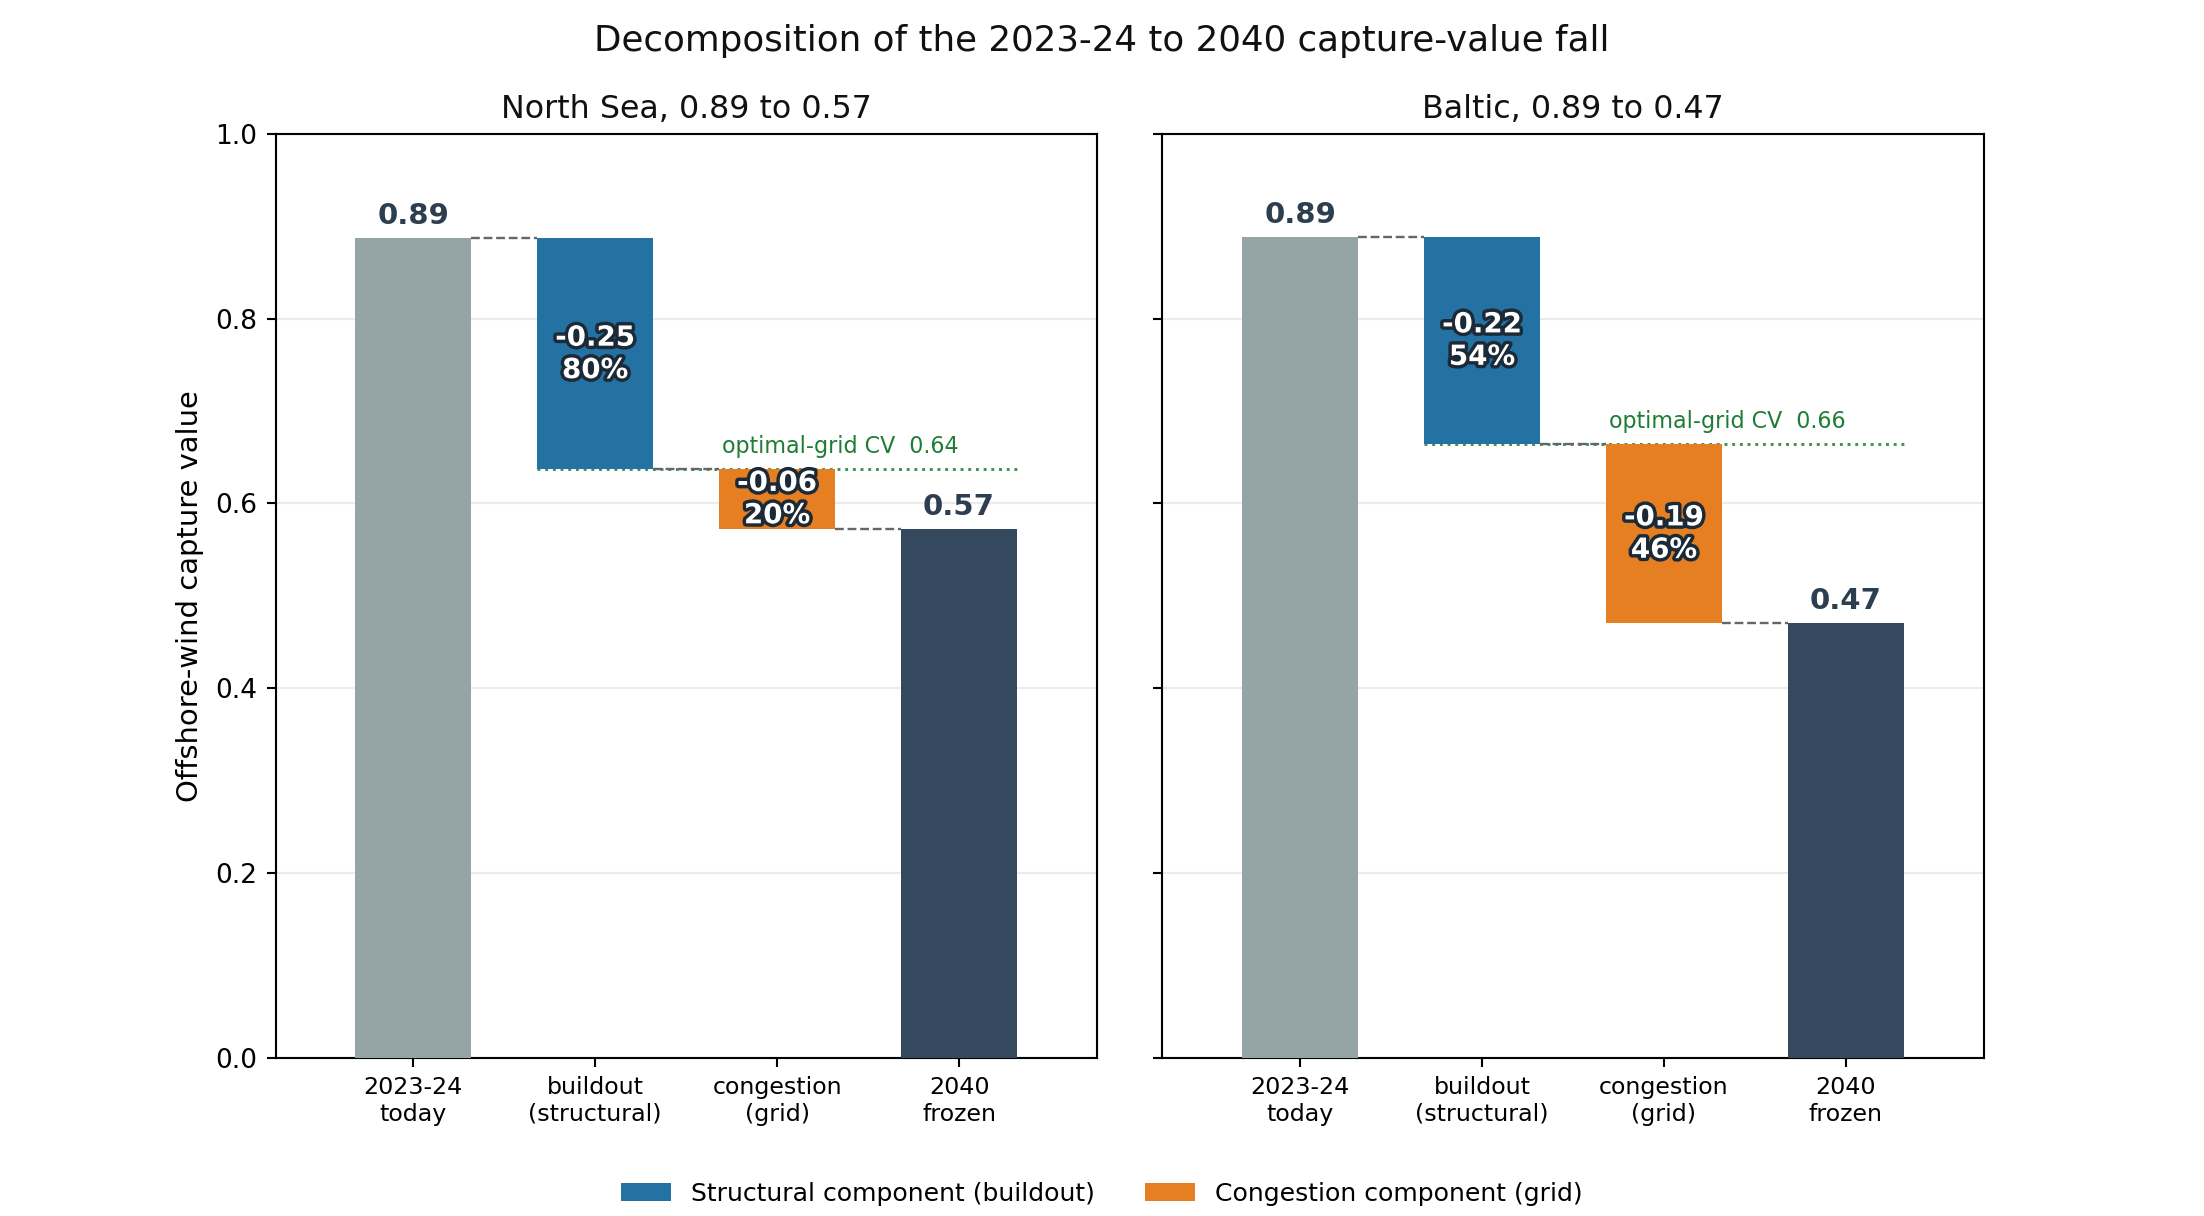
\includegraphics[width=0.94\textwidth]{fig_cv_decomposition}
    \caption{Each basin's fall in capture value between today and 2040, divided
    into the part caused by the buildout itself, which no amount of transmission
    removes, and the part caused by congestion, which an expanded grid removes.
    Both basins start at about 0.89.}
    \label{fig:cv_decomposition}
\end{figure}

The Baltic's congestion penalty is three times the North Sea's, which is what an
enclosed basin should show. The more surprising result is the structural fall:
at 0.225 against the North Sea's 0.250, the part no transmission can recover is
the smaller of the two. The share of the Baltic's disadvantage that appears to
come from enclosure is congestion, and congestion is decided by what
is built. How the two components differ in who pays for them, while they remain,
is taken up in Section~\ref{sec:whopays_results}.

\subsection{Value-adjusted cost of energy and site selection}\label{sec:vlcoe_results}

The chapter has measured capture value and explained why it falls. This section
turns it into the number an investor uses. Combining capture value with the
levelised cost of energy (Equation~\ref{eq:vlcoe}) gives the average wholesale
price a site must earn over its life to break even, and that price is mapped
across both basins at the same resolution as the wind and seabed data.

\subsubsection{Levelised cost and the break-even price}\label{sec:vlcoe_paradox}

Building offshore wind is getting cheaper. Across the seabed where farms could
be built, the median levelised cost falls from 74 to 66~\euro/MWh between 2025
and 2040. The price a site must earn to break even moves the other way, rising
from 87 to 121~\euro/MWh (Figure~\ref{fig:vlcoe}), because capture value falls
faster than cost does. The share of that seabed clearing a market price near
70~\euro/MWh falls from about 35 per cent to under 1 per cent.

Cheaper turbines do not save the economics, because offshore wind keeps
improving when measured per megawatt-hour produced, yet gets worse when
measured per megawatt-hour of value delivered, and it is the second that a
merchant project, one selling at market prices without a support contract, is
paid for.

\begin{figure}[!htb]
    \centering
    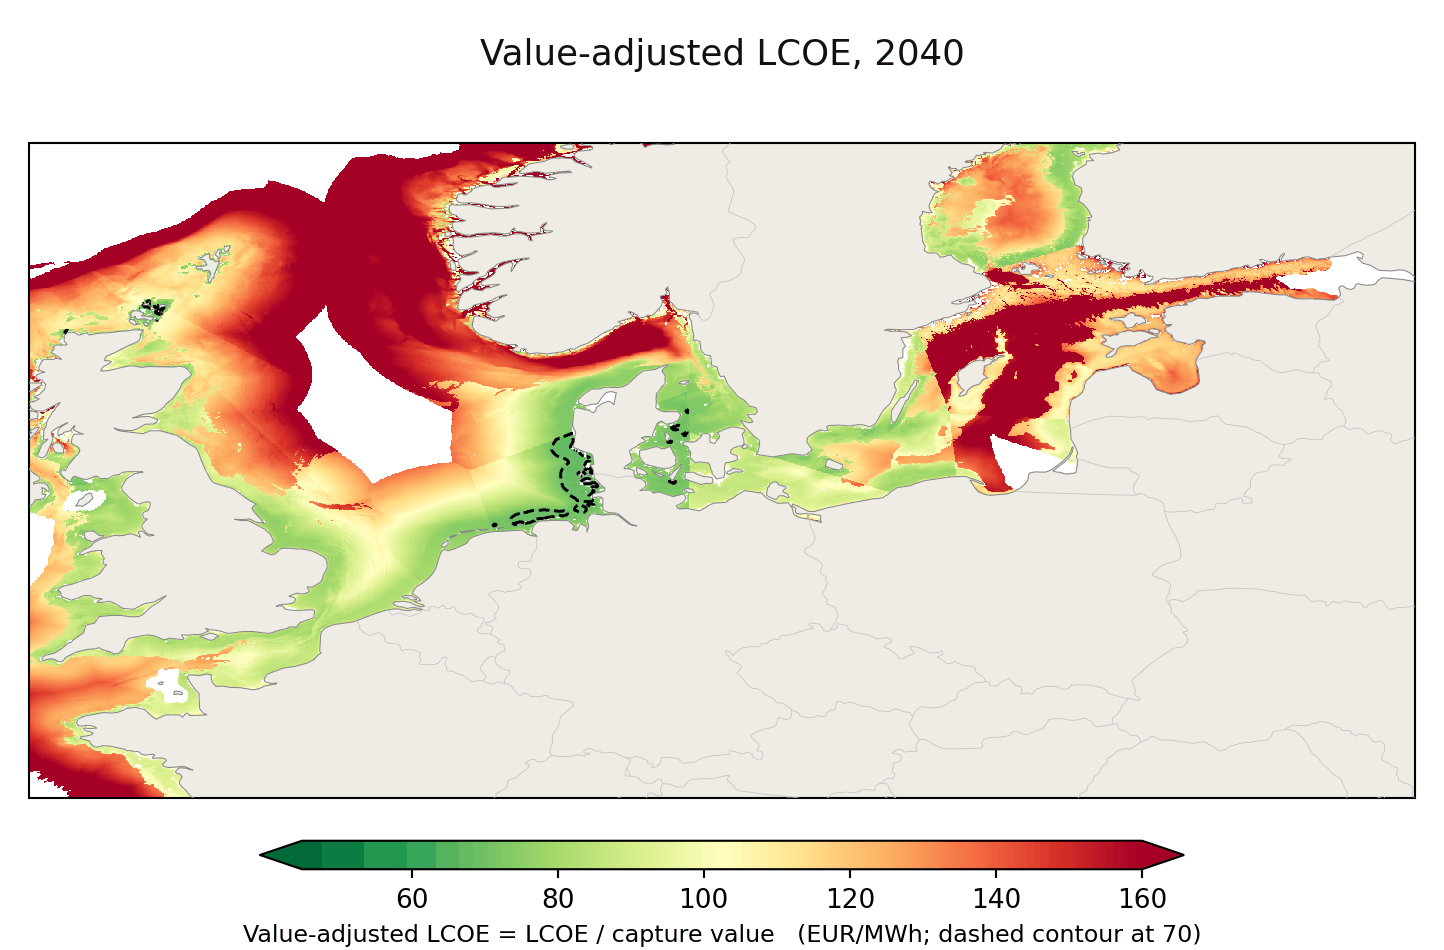
\includegraphics[width=0.6\textwidth]{fig_vlcoe_2040}
    \caption{The average wholesale price each site must earn to break even in
    2040, calculated as levelised cost divided by capture value. The dashed
    contour marks a market price of about 70~\euro/MWh; sites inside it are
    viable at that price.}
    \label{fig:vlcoe}
\end{figure}

The direction does not depend on the cost assumptions. Across all 27
combinations of discount rate, capital cost and learning rate, the break-even
price rises to 2040 in every case (Figure~\ref{fig:vlcoe_robust}). The reason is
that the cost level cancels out: the break-even price is cost divided by capture
value, so what decides the direction is only whether cost falls faster than
value. For the break-even price to stay level, offshore capital costs would have
to fall by about 36 per cent by 2040, three times what the cost database
projects.

Comparing the revenue a farm captures against its annual cost gives the same
picture in absolute terms\label{sec:netvalue_results}. About 48 per cent of the
buildable seabed is profitable at market prices in 2025, and roughly 12 per cent
by 2040. Falling value drives that shrinkage, since costs are falling over the
same period (Appendix~\ref{app:atlas}).

\subsubsection{Monetised value of interconnection}\label{sec:vlcoe_grid_results}

The break-even price is levelised cost divided by capture value, so the grid
result of Section~\ref{sec:grid_results} reappears in terms of money. The 2040
break-even price was recalculated with the frozen and the expanded capture
values, holding offshore cost identical in both. Expansion lowers it everywhere,
and four times more in the enclosed Baltic than in the open North Sea: by about
8~\euro/MWh in the North Sea, by 33 in the enclosed Baltic, and by 48 in the
Danish corridor that carries the redirected flows
(Figure~\ref{fig:vlcoe_grid}).

In revenue terms the Baltic gain alone is worth roughly 1.2 billion euros a
year, close to half the annual cost of the whole transmission programme, and
that is before the congestion rent of Section~\ref{sec:rent_results} is counted.
Interconnection therefore cuts the break-even price where the cut is most
needed.

\begin{figure}[!htb]
    \centering
    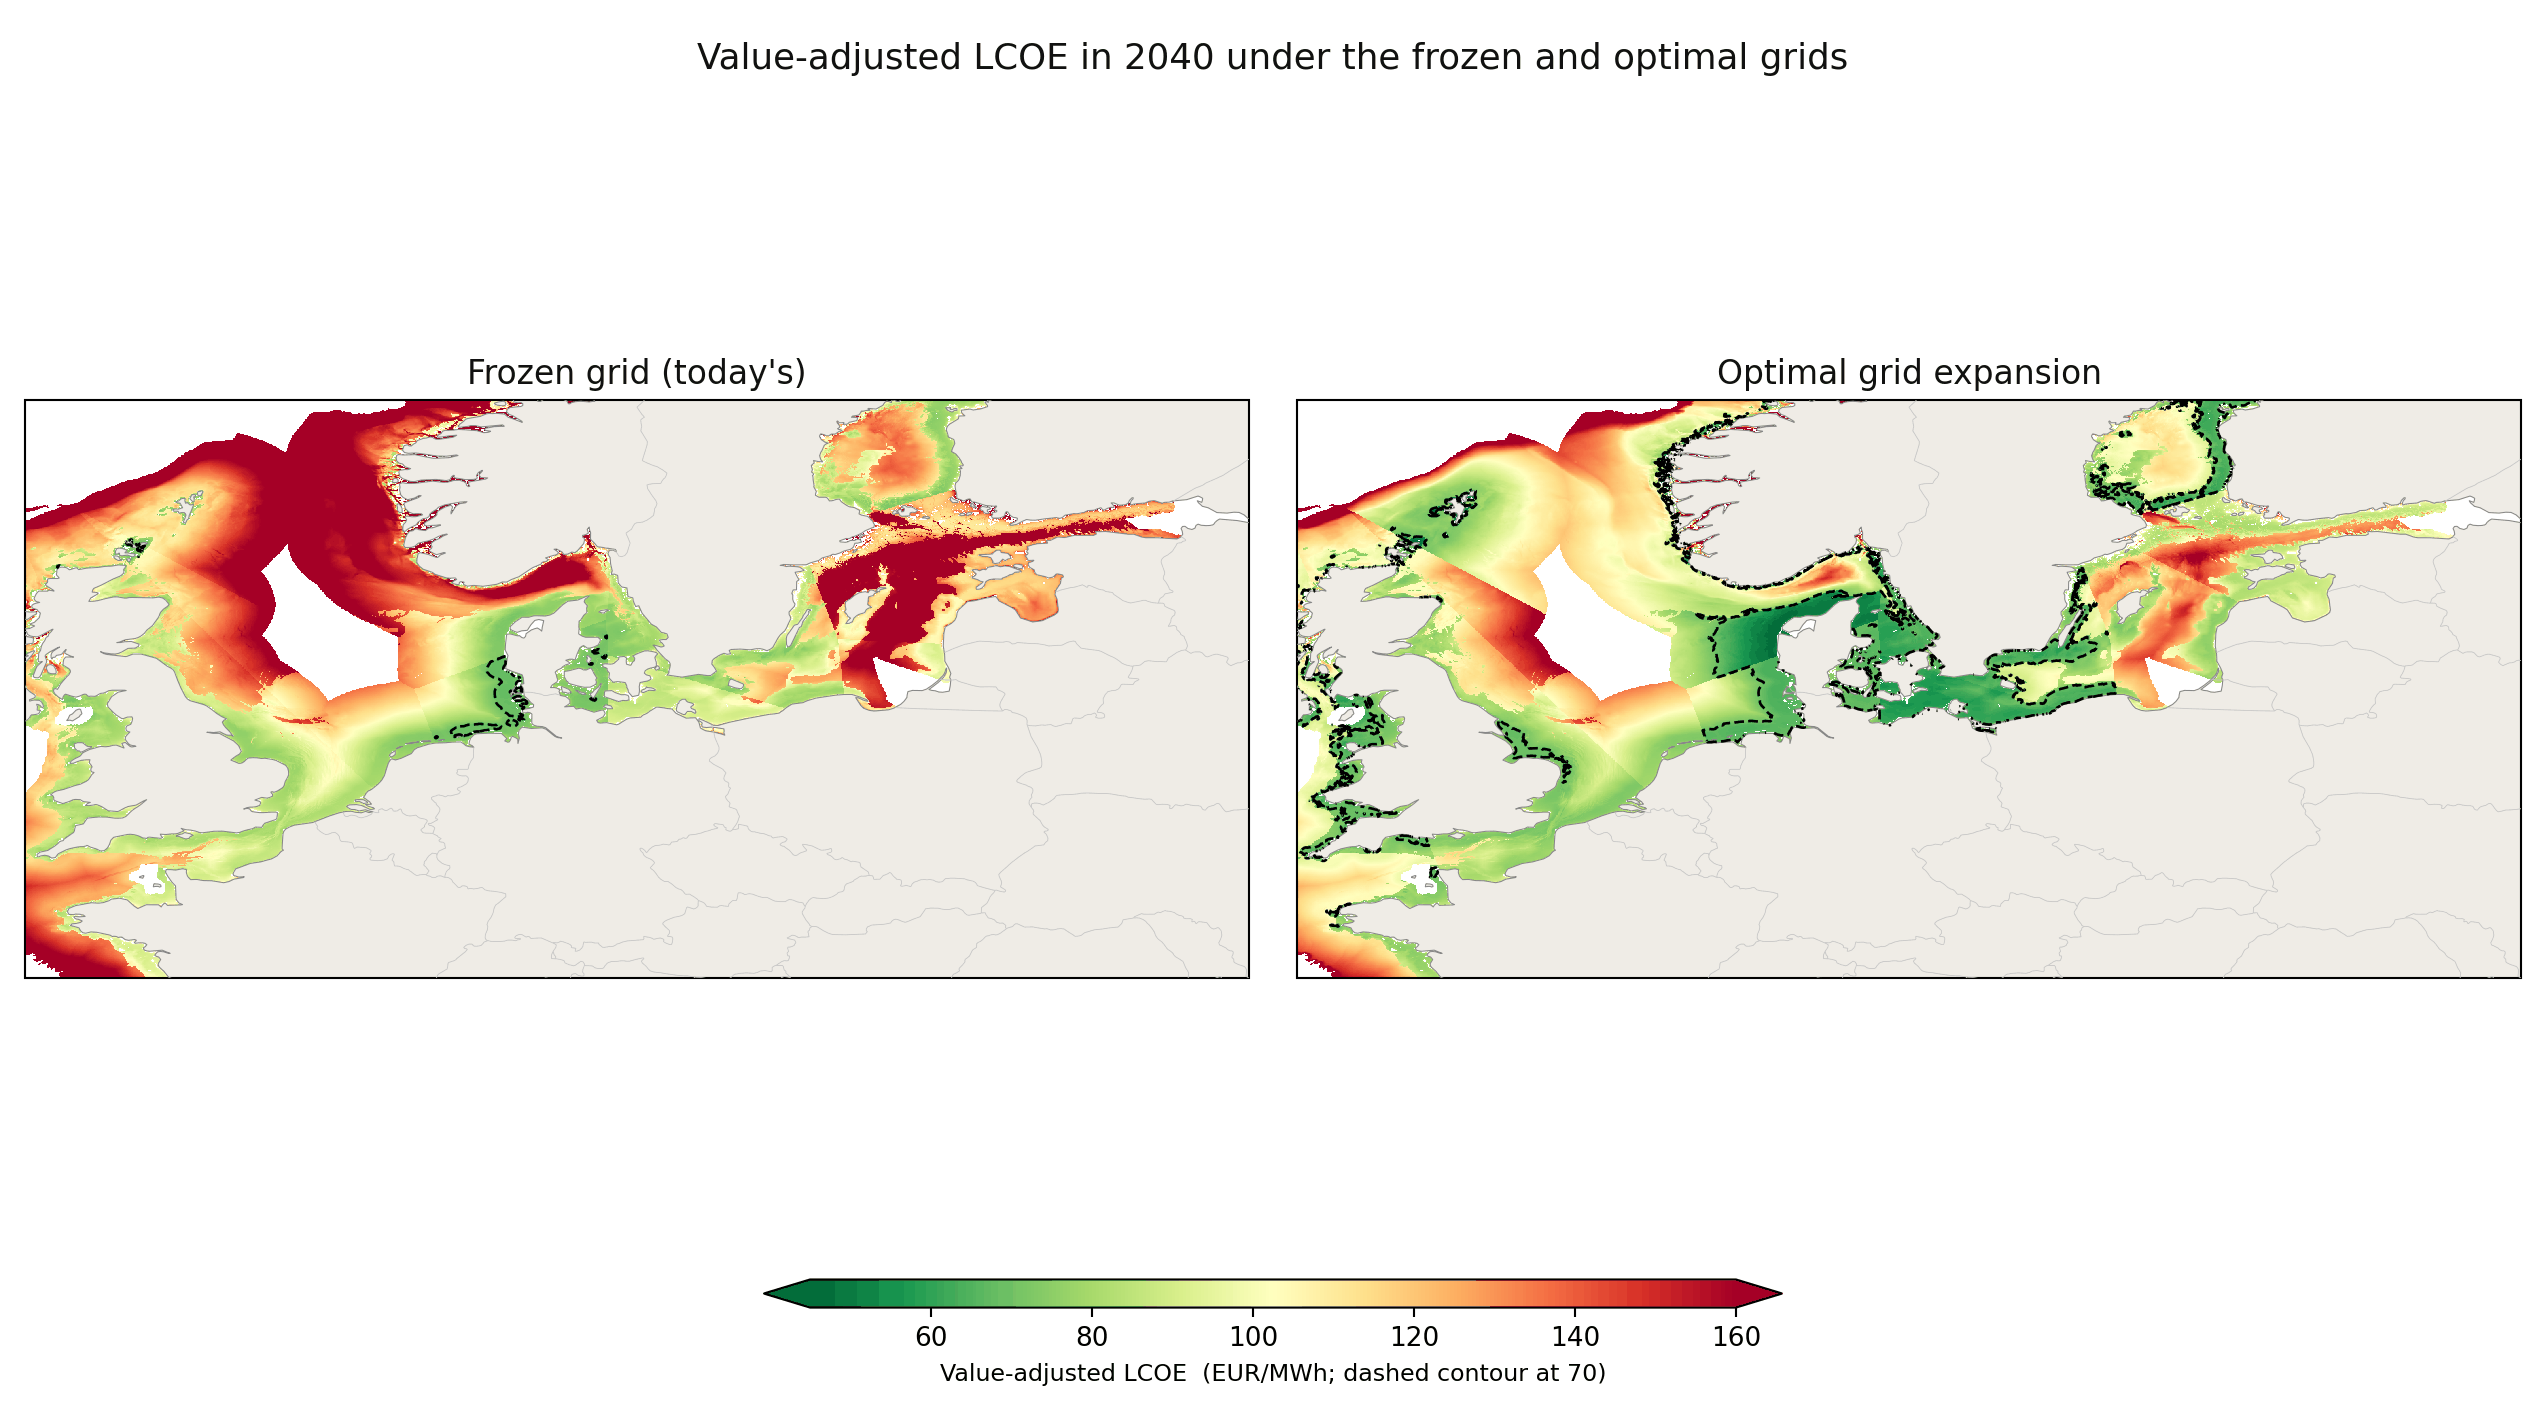
\includegraphics[width=0.96\textwidth]{fig_vlcoe_grid_2040}
    \caption{The 2040 break-even price with the transmission grid held at
    today's capacity (left) and free to expand (right), with offshore cost
    identical in both. The price falls most where the Baltic is enclosed.}
    \label{fig:vlcoe_grid}
\end{figure}

\subsubsection{Effect of capture value on site ranking}\label{sec:site_ranking}

Ten candidate development areas, one in each offshore bidding zone, were ranked
twice in each year: once on levelised cost alone, and once on the break-even
price that includes capture value. Comparing the two orderings shows how much
capture value changes where a developer would build
(Figure~\ref{fig:site_ranking}).

\begin{figure}[!htb]
    \centering
    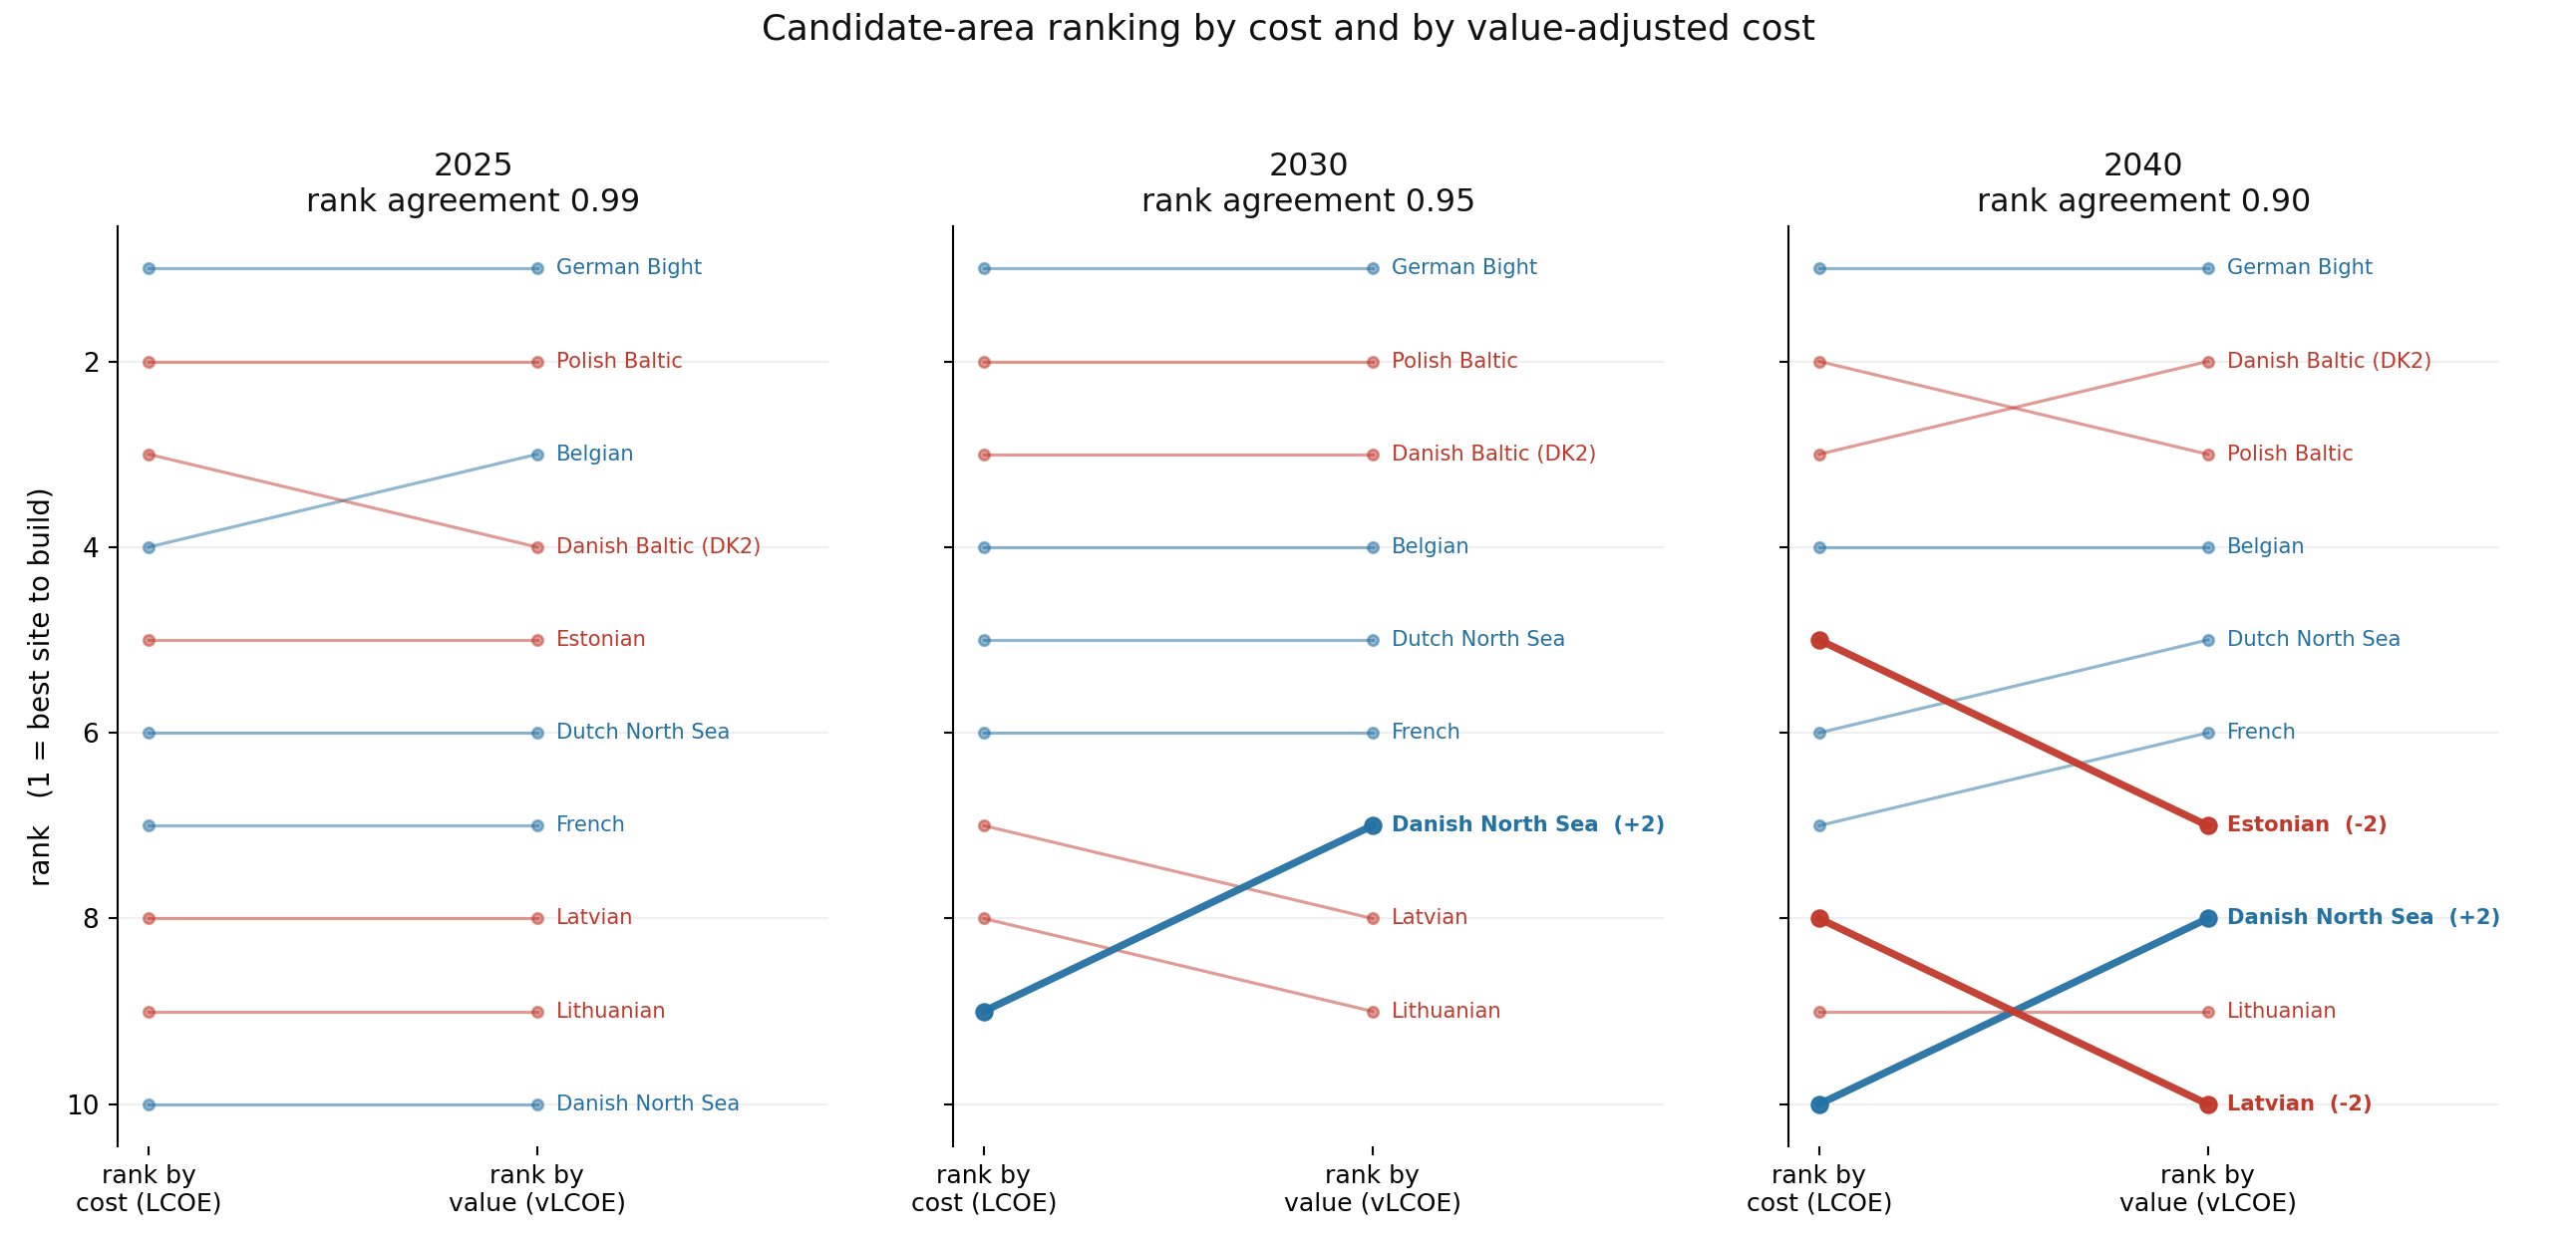
\includegraphics[width=0.94\textwidth]{fig_site_ranking}
    \caption{Candidate development areas ranked on cost alone against the
    break-even price, 2025 to 2040. Areas that hold their position lie on the
    diagonal, and bold lines mark moves of two places or more, in blue for the
    North Sea and red for the Baltic.}
    \label{fig:site_ranking}
\end{figure}

The ranking by levelised cost alone and the ranking by break-even price agree
almost perfectly today and drift apart over time, with a rank correlation of
0.99 in 2025, 0.95 in 2030 and 0.90 by 2040 (Appendix~\ref{app:tables}).
Ranking on cost alone is therefore adequate for a project being built now, and
increasingly misleading for one being built into the 2040s, which is the
period over which offshore wind is financed.

The individual movements identify the misranked areas, and the clearest case
is the cheap eastern Baltic: Estonia has one of the lowest levelised costs on the shelf at 51~\euro/MWh, but
at a capture value of 0.39 its break-even price is 130~\euro/MWh. The Danish
areas rise, because their capture value holds up. The German Bight ranks first
on both measures in every year, having the strongest wind in shallow water close
to shore.

Widening the comparison to 169 candidate locations across both seas gives the
same answer. Whether areas are judged on value for money or on absolute profit,
the German Bight and the shallow western Baltic come first, and the cheap
eastern Baltic scores well on cost and poorly on value
(Appendix~\ref{app:atlas}).

Cost alone remains a defensible basis for the current round of projects,
and a progressively worse one as the buildout advances, with the error
concentrated in the cheap eastern Baltic sites it would promote.

Who bears the resulting loss is a separate question, worked through in
Appendix~\ref{app:portfolio}. Splitting each basin's loss into the part a
support contract absorbs and the part it does not shows that the two basins
differ beneath similar headline numbers: 18.5\,\% of Baltic energy on today's
grid earns nothing at all, while the whole of the North Sea's loss falls outside
what a contract compensates. Building the grid both reduces the loss and changes
who carries it.

% ----------------------------------------------------------------------------
